\documentclass[a4paper]{article}
\usepackage[a4paper]{geometry}
\usepackage[utf8]{inputenc}

\usepackage{amsmath,amsfonts,amssymb,amsthm}
\usepackage{thmtools}
\usepackage{stmaryrd}
\usepackage{natbib}
\usepackage{url}
\usepackage{array}
\usepackage{arydshln}
\usepackage{ifthen}
\usepackage{ifpdf}
\usepackage{verbatim}
\usepackage{mathpartir}
\usepackage{listings}
\lstset{
  basicstyle=\ttfamily,
  columns=fullflexible,
  keepspaces=true,
  mathescape
}

\usepackage{rotating}

\usepackage{mathtools}
\DeclarePairedDelimiter\ceil{\lceil}{\rceil}
\DeclarePairedDelimiter\floor{\lfloor}{\rfloor}

\usepackage{appendix}

\usepackage{enumitem}
\newlist{enumproof}{enumerate}{10}
\setlist[enumproof]{label*=\arabic*.}

\usepackage{tikz}
\usepackage{multirow,bigdelim}

%% make latex preview-mode work with natbib...
%\usepackage[displaymath,floats,graphics,textmath,footnotes]{preview}

\declaretheorem[numbered=yes,name=Lemma,qed=$\blacksquare$]{lemma}
\declaretheorem[numbered=yes,name=Definition,qed=$\blacksquare$]{definition}
\declaretheorem[numbered=yes,name=Specification,qed=$\blacksquare$]{specification}

\newcommand{\forcenewline}{$\phantom{v}$\\}
\newcommand{\judgment}[2]{\paragraph{#1}\hspace{\stretch{1}}\fbox{$#2$}}

\newcommand{\update}[2]{[#1 \mapsto #2]}
\newcommand{\sem}[1]{\left\llbracket #1 \right\rrbracket}

% Math notation
\newcommand{\restrictfun}[1]{|_{#1}}
\newcommand{\parfun}{\rightharpoonup}
\newcommand{\finparfun}{\xrightharpoonup{\textit{\tiny{fin}}}}
\newcommand{\monnefun}{\xrightarrow{\textit{\tiny{mon, ne}}}}
\newcommand{\monfun}{\xrightarrow{\textit{\tiny{mon}}}}
\newcommand{\nefun}{\xrightarrow{\textit{\tiny{ne}}}}
\newcommand{\fun}{\rightarrow}
\newcommand{\defeq}{\stackrel{\textit{\tiny{def}}}{=}}
\newcommand{\nequal}[1][n]{\stackrel{\tiny{#1}}{=}}
\renewcommand{\nsim}[1][n]{\stackrel{\tiny{#1}}{\simeq}}

\newcommand\subsetsim{\mathrel{\ooalign{\raise.2ex\hbox{$\subset$}\cr
      \hidewidth\lower.8ex\hbox{\scalebox{0.9}{$\sim$}}\hidewidth\cr}}}
\newcommand\supsetsim{\mathrel{\ooalign{\raise.2ex\hbox{$\supset$}\cr
      \hidewidth\lower.8ex\hbox{\scalebox{0.9}{$\sim$}}\hidewidth\cr}}}
\newcommand{\nsubsim}[1][n]{\stackrel{\tiny{#1}}{\subsetsim}}
\newcommand{\nsupsim}[1][n]{\stackrel{\tiny{#1}}{\supsetsim}}

\newcommand{\nsubeq}[1][n]{\stackrel{\tiny{#1}}{\subseteq}}
\newcommand{\nsupeq}[1][n]{\stackrel{\tiny{#1}}{\supseteq}}

\newcommand{\union}{\mathbin{\cup}}
\DeclareMathOperator{\dom}{dom}
\newcommand{\blater}{\mathop{\blacktriangleright}}
\newcommand{\id}{\var{id}}
\newcommand{\undefined}{\mathit{undefined}}

\newcommand{\powerset}[1]{\mathcal{P}(#1)}

\newcommand{\false}{\mathit{false}}
\newcommand{\true}{\mathit{true}}


% cofes
\newcommand{\cofe}{c.o.f.e.}
\newcommand{\cofes}{\cofe{}'s}
\newcommand{\CatC}{\mathbb{C}}
\newcommand{\CatP}{\mathbb{P}}

% Comments
\newcommand\lau[1]{{\color{purple} \sf \footnotesize {LS: #1}}\\}
\newcommand\dominique[1]{{\color{purple} \sf \footnotesize {DD: #1}}\\}
\newcommand\lars[1]{{\color{purple} \sf \footnotesize {LB: #1}}\\}

% Variables
\newcommand{\var}[1]{\mathit{#1}}
\newcommand{\hs}{\var{ms}}
\newcommand{\ms}{\hs}
\newcommand{\hv}{\var{hv}}
\newcommand{\rv}{\var{rv}}
\newcommand{\lv}{\var{lv}}
\newcommand{\gl}{\var{g}}
\newcommand{\pc}{\mathit{pc}}
\newcommand{\pcreg}{\mathrm{pc}}
\newcommand{\addr}{\var{a}}
\newcommand{\offset}{\var{offset}}
\newcommand{\word}{\var{w}}
\newcommand{\start}{\var{base}}
\newcommand{\addrend}{\var{end}}
\newcommand{\pwlv}{\var{pwl}}
\newcommand{\mem}{\var{mem}}
\newcommand{\reg}{\var{reg}}
\newcommand{\heapseg}{\var{ms}}
\newcommand{\heap}{\var{mem}}
\newcommand{\mode}{\var{mode}}
\newcommand{\perm}{\var{perm}}
\newcommand{\permp}{\var{permPair}}
\newcommand{\roll}{\var{roll}}
\newcommand{\instr}{\var{instr}}
\newcommand{\stdcap}[1][(\perm,\gl)]{\left(#1,\start,\addrend,\addr \right)}
\newcommand{\adv}{\var{adv}}
\newcommand{\msframe}{ms_\var{frame}}
\newcommand{\link}{\var{link}}
\newcommand{\stk}{\var{stk}}
\newcommand{\flag}{\var{flag}}
\newcommand{\nwl}{\var{nwl}}
\newcommand{\pwl}{\var{pwl}}
\newcommand{\sta}{\var{sta}}
\newcommand{\cnst}{\var{cnst}}
\newcommand{\olf}{\var{offsetLinkFlag}}
\newcommand{\prp}{\var{prp}}

% Memory projections
\newcommand{\plainproj}[1]{\mathrm{#1}}
\newcommand{\memheap}[1][\Phi]{#1.\plainproj{mem}}
\newcommand{\memreg}[1][\Phi]{#1.\plainproj{reg}}

\newcommand{\updateHeap}[3][\Phi]{#1\update{\plainproj{mem}.#2}{#3}}
\newcommand{\updateReg}[3][\Phi]{#1\update{\plainproj{reg}.#2}{#3}}

% Configuration end states
\newcommand{\failed}{\textsl{failed}}
\newcommand{\halted}{\textsl{halted}}

% Functions
\newcommand{\plainfun}[2]{
  \ifthenelse{\equal{#2}{}}
  {\mathit{#1}}
  {\mathit{#1}(#2)}
}
\newcommand{\decode}{\plainfun{decode}{}}
\newcommand{\encode}{\plainfun{encode}{}}
\newcommand{\encodePerm}{\mathit{encodePerm}}
\newcommand{\encodePermPair}{\plainfun{encodePermPair}{}}
\newcommand{\encodeLoc}{\mathit{encodeLoc}{}}
\newcommand{\decodePermPair}{\plainfun{decodePermPair}}
\newcommand{\decodePerm}[1]{\plainfun{decodePerm}{#1}}
\newcommand{\updatePcPerm}[1]{\plainfun{updatePcPerm}{#1}}

\newcommand{\executeAllowed}[1]{\plainfun{executeAllowed}{#1}}
\newcommand{\nonZero}[1]{\plainfun{nonZero}{#1}}
\newcommand{\readAllowed}[1]{\plainfun{readAllowed}{#1}}
\newcommand{\writeAllowed}[1]{\plainfun{writeAllowed}{#1}}
\newcommand{\withinBounds}[1]{\plainfun{withinBounds}{#1}}
\newcommand{\stdUpdatePc}[1]{\plainfun{updatePc}{#1}}

\newcommand{\readCond}[1]{\plainfun{readCondition}{#1}}
\newcommand{\writeCond}[1]{\plainfun{writeCondition}{#1}}
\newcommand{\execCond}[1]{\plainfun{executeCondition}{#1}}
\newcommand{\entryCond}[1]{\plainfun{enterCondition}{#1}}

\newcommand{\revokeTemp}[1]{\plainfun{revokeTemp}{#1}}
\newcommand{\erase}[2]{\floor*{#1}_{\{#2\}}}
\newcommand{\activeReg}[1]{\plainfun{active}{#1}}

% World operations
\newcommand{\future}{\mathbin{\sqsupseteq}}
\newcommand{\futurewk}{\mathbin{\sqsupseteq}^{\var{pub}}}
\newcommand{\futurestr}{\mathbin{\sqsupseteq}^{\var{priv}}}
\newcommand{\heapSat}[3][\heap]{#1 :_{#2} #3}
\newcommand{\memSat}[3][n]{\heapSat[#2]{#1}{#3}}
\newcommand{\memSatPar}[4][n]{\heapSat[#2]{#1 , #4}{#3}}

\newcommand{\monwknefun}{\xrightarrow[\text{\tiny{$\futurewk$}}]{\textit{\tiny{mon, ne}}}}
\newcommand{\monstrnefun}{\xrightarrow[\text{\tiny{$\futurestr$}}]{\textit{\tiny{mon, ne}}}}


% Assembly labels
\newcommand{\codelabel}[1]{\mathit{#1}}
\newcommand{\init}{\codelabel{init}}
\newcommand{\malloc}{\codelabel{malloc}}
\newcommand{\counter}{\codelabel{counter}}
\newcommand{\iocap}{\codelabel{iocap}}

% Type(s)
\newcommand{\type}[1]{\mathrm{#1}}
\newcommand{\asmType}{\plaindom{AsmType}}


% Domains
\newcommand{\plaindom}[1]{\mathrm{#1}}
\newcommand{\Caps}{\plaindom{Cap}}
\newcommand{\Words}{\plaindom{Word}}
\newcommand{\Addrs}{\plaindom{Addr}}
\newcommand{\ExecConfs}{\plaindom{ExecConf}}
\newcommand{\RegName}{\plaindom{RegisterName}}
\newcommand{\Regs}{\plaindom{Reg}}
\newcommand{\Heaps}{\plaindom{Mem}}
\newcommand{\Mems}{\Heaps}
\newcommand{\HeapSegments}{\plaindom{MemSegment}}
\newcommand{\MemSegments}{\HeapSegments}
\newcommand{\Confs}{\plaindom{Conf}}
\newcommand{\Instrs}{\plaindom{Instructions}}
\newcommand{\nats}{\mathbb{N}}
\newcommand{\ints}{\mathbb{Z}}
\newcommand{\Perms}{\plaindom{Perm}}
\newcommand{\Globals}{\plaindom{Global}}

\newcommand{\Rel}{\plaindom{Rel}}
\newcommand{\States}{\plaindom{State}}
\newcommand{\RegionNames}{\plaindom{RegionName}}
\newcommand{\Regions}{\plaindom{Region}}
\newcommand{\Reg}{\plaindom{Reg}}
\newcommand{\Worlds}{\plaindom{World}}
\newcommand{\Wor}{\plaindom{Wor}}
\newcommand{\Worwk}{\Wor_{\futurewk}}
\newcommand{\Worstr}{\Wor_{\futurestr}}
\newcommand{\xiwk}{\xi_{\var{wk}}}
\newcommand{\xistr}{\xi_{\var{str}}}
\newcommand{\StorePred}{\plaindom{MemSegPred}}
\newcommand{\UPred}[1]{\plaindom{UPred}(#1)}
\newcommand{\DCPred}[1]{\plaindom{P}^\downarrow(#1)}

\newcommand{\Views}{\plaindom{View}}

% LR
\newcommand{\intr}[2]{\mathcal{#1}}
\newcommand{\valueintr}[1]{\intr{V}{#1}}
\newcommand{\exprintr}[1]{\intr{E}{#1}}
\newcommand{\contintr}[1]{\intr{K}{#1}}
\newcommand{\regintr}[1]{\intr{R}{#1}}
\newcommand{\stdvr}{\valueintr{\asmType}}
\newcommand{\stder}{\exprintr{\asmType}}
\newcommand{\stdrr}{\regintr{\asmType}}
\newcommand{\stdkr}{\contintr{\asmType}}
\newcommand{\observations}{\mathcal{O}}
\newcommand{\npair}[2][n]{\left(#1,#2 \right)}

% Reference register/memory
\newcommand{\refreg}[1]{\lfloor #1 \rfloor}
\newcommand{\refheap}[1]{\langle #1 \rangle_m}

% Instructions
% No arguments
\newcommand{\zinstr}[1]{\mathtt{#1}}
\newcommand{\fail}{\zinstr{fail}}
\newcommand{\halt}{\zinstr{halt}}
% One argument
\newcommand{\oneinstr}[2]{\zinstr{#1} \; #2}
\newcommand{\jmp}[1]{\oneinstr{jmp}{#1}}
% Two arguments
\newcommand{\twoinstr}[3]{\zinstr{#1} \; #2 \; #3}
\newcommand{\restricttwo}[2]{\twoinstr{restrict}{#1}{#2}}
\newcommand{\jnz}[2]{\twoinstr{jnz}{#1}{#2}}
\newcommand{\isptr}[2]{\twoinstr{isptr}{#1}{#2}}
\newcommand{\geta}[2]{\twoinstr{geta}{#1}{#2}}
\newcommand{\getb}[2]{\twoinstr{getb}{#1}{#2}}
\newcommand{\gete}[2]{\twoinstr{gete}{#1}{#2}}
\newcommand{\getp}[2]{\twoinstr{getp}{#1}{#2}}
\newcommand{\getl}[2]{\twoinstr{getl}{#1}{#2}}
\newcommand{\move}[2]{\twoinstr{move}{#1}{#2}}
\newcommand{\store}[2]{\twoinstr{store}{#1}{#2}}
\newcommand{\load}[2]{\twoinstr{load}{#1}{#2}}
\newcommand{\lea}[2]{\twoinstr{lea}{#1}{#2}}
% Three arguments
\newcommand{\threeinstr}[4]{\zinstr{#1} \; #2 \; #3 \; #4}
\newcommand{\restrict}[3]{\threeinstr{restrict}{#1}{#2}{#3}}
\newcommand{\subseg}[3]{\threeinstr{subseg}{#1}{#2}{#3}}
\newcommand{\plus}[3]{\threeinstr{plus}{#1}{#2}{#3}}

% Permissions
\newcommand{\plainperm}[1]{\mathrm{#1}}
\newcommand{\noperm}{\plainperm{o}}
\newcommand{\readonly}{\plainperm{ro}}
\newcommand{\readwrite}{\plainperm{rw}}
\newcommand{\exec}{\plainperm{rx}}
\newcommand{\entry}{\plainperm{e}}
\newcommand{\rwx}{\plainperm{rwx}}
% PWL permissions
\newcommand{\readwritel}{\plainperm{rwl}}
\newcommand{\rwl}{\readwritel}
\newcommand{\rwlx}{\plainperm{rwlx}}

% Global/local
\newcommand{\local}{\plainperm{local}}
\newcommand{\glob}{\plainperm{global}}

\newcommand{\localityReg}{\var{localityReg}}
\newcommand{\localReg}{\var{localReg}}
\newcommand{\globalReg}{\var{globalReg}}

% Views
\newcommand{\plainview}[1]{\mathrm{#1}}
\newcommand{\perma}{\plainview{perm}}
\newcommand{\temp}{\plainview{temp}}
\newcommand{\revoked}{\plainview{revoked}}

% OP sem
\newcommand{\diverge}[1][n]{\not\Downarrow_{#1}}
\newcommand{\step}[1][]{\rightarrow_{#1}}

% Conv defs
\newcommand{\lookingat}[3]{\ensuremath{#1} \text{ is looking at } \ensuremath{#2} \text{ followed by } \ensuremath{#3}}
\newcommand{\pointstostack}[3]{\ensuremath{#1} \text{ points to stack with } \ensuremath{#2} \text{ used and } \ensuremath{#3} \text{ unused}}

% Macros
\newcommand{\scall}[3]{\mathtt{scall} \; #1(#2,#3)}


\begin{document}
\begin{flushright}
  \today
\end{flushright}
\section{Domains and Notation}

\begin{align*}
  \Addrs &::= \nats\\
  \Words &::= \Caps + \ints \\
  \Regs  &::= \RegName \rightarrow \Words\\
  \Heaps &::= \Addrs \rightarrow \Words \\
  \Perms &::= \{ \noperm, \readonly, \readwrite, \readwritel, \exec, \entry, \rwx, \rwlx\}\\
  \ExecConfs  &::= \Regs \times \Heaps \\
  \Globals & ::= \{\glob, \local \} \\
  \Caps  &::= (\Perms \times \Globals) \times \Addrs \times (\Addrs + \{ \infty \}) \times \Addrs\\
  \Confs &::= \ExecConfs + \{\failed \} + \halted \times \ExecConfs \\
  \HeapSegments &::= \Addrs \parfun \Words
\end{align*}
Local capabilities have been added by adding a new domain $\Globals$ which represents whether a capability is local or global. There are two new permissions $\readwritel$ and $\rwlx$ that permits writing local capabilities. They are otherwise the same as their non-''permit write local'' counterparts.

\begin{figure}[!h]
  \centering
  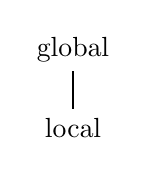
\begin{tikzpicture}[main node/.style={}]
    \node[main node] (1) {$\glob$};
    \node[main node] (2) [below of=1] {$\local$};

    \path[every node/.style={font=\sffamily\small}]
    (1) edge (2);
  \end{tikzpicture}
  \caption{Permission hierarchy}
  \label{fig:glob-hier}
\end{figure}

Things to note:
\begin{itemize}
\item $\RegName$ contains $\pcreg$, but is otherwise a sufficiently
  large finite set.
\item Table~\ref{tab:permission-list} describes what all the permissions grant access to.
\item Figure~\ref{fig:perm-hier} shows the ordering of the permissions, i.e, the elements of $\Perms$.
\item Figure~\ref{fig:glob-hier} shows the ordering of $\local$ and $\glob$, i.e., the elements of $\Globals$.
\item The ordering of $\Perms \times \Globals$ is pointwise.
\end{itemize}

\begin{table}[!h]
  \centering
  \begin{tabular}[!h]{r |  p{7cm} }
    $\noperm$ & No permissions. Grants no permissions\\
    \hline
    $\readonly$ & Read only. Grants read permission \\
    \hline
    $\readwrite$ & Read-write. Grants read and write permission. Storage of local capabilities prohibited. \\
    \hline
    $\readwritel$ & Read-write, permit write local. Grants read and write permission. Storage of local capabilities possible. \\
    \hline
    $\exec$ & Execute permission. Grants execute and read permissions.\\
    \hline
    $\entry$ & Enter permission. This permission grants no access, but when jumped to, it will turn into an $\exec$ permission.\\
    \hline
    $\rwx$ & Read-write-execute permission. Grants read, write, and execute permissions. Storage of local capabilities prohibited. \\
    \hline
    $\rwlx$ & Read-write-execute, permit write local. Grants read, write, and execute permissions. Storage of local capabilities possible.
  \end{tabular}

  \caption{The permissions in this capability system}
  \label{tab:permission-list}
\end{table}
\begin{figure}[!h]
  \centering
  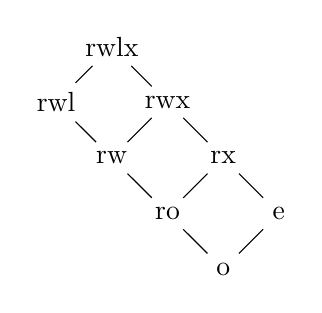
\begin{tikzpicture}[main node/.style={}]
    \node[main node] (7) {$\rwlx$};
    \node[main node] (8) [below left of=7] {$\readwritel$};
    \node[main node] (1) [below right of=7] {$\rwx$};
    \node[main node] (2) [below right of=1] {$\exec$};
    \node[main node] (3) [below right of=2] {$\entry$};
    \node[main node] (4) [below left of=1] {$\readwrite$};
    \node[main node] (5) [below right of=4] {$\readonly$};
    \node[main node] (6) [below right of=5] {$\noperm$};

    \path[every node/.style={font=\sffamily\small}]
    (7) edge (8)
    (7) edge (1)
    (8) edge (4)
    (1) edge (2)
    (2) edge (3)
    (2) edge (5)
    (3) edge (6)
    (1) edge (4)
    (4) edge (5)
    (5) edge (6);
  \end{tikzpicture}

  \caption{Permission hierarchy}
  \label{fig:perm-hier}
\end{figure}
Notation:
\[
  \begin{array}{rcl}
    i       &\in& \Instrs \\
    r       &\in& \RegName\\
    \pc     &\in& \Caps \\
    \pcreg  &\in& \RegName \\
    \Phi    &\in& \ExecConfs \\
    m, \memheap&\in& \Heaps \\
    \memreg &\in& \Regs \\
    \addr   &\in& \Addrs\\
    \perm   &\in& \Perms\\
    ((\perm,\gl),\start,\addrend,\addr) &\in& \Caps \\
    n       &\in& \ints\\
    \ms     &\in& \MemSegments
  \end{array}
\]
Words and instructions:
\[
  \begin{array}{rcl}
    \lv    &::=& \refreg{r} \\
    \hv    &::=& \refheap{r}\\
    \rv    &::=& n \mid \lv \\
    i      &::=& 
                 \jmp{\lv} \mid 
                 \jnz{\lv}{\rv} \mid
                 \move{\lv}{\rv} \mid 
                 \load{\lv}{\hv} \mid 
                 \store{\hv}{\rv} \mid  \\
           &   & \plus{\lv}{\rv}{\rv} \mid 
                 \lea{\lv}{\rv} \mid 
                 \restricttwo{\lv}{\rv} \mid 
                 \subseg{\lv}{\rv}{\rv} \mid  \\
           &   & \isptr{\lv}{\rv} \mid 
                 \getp{\lv}{\lv} \mid 
                 \getl{\lv}{\lv} \mid 
                 \getb{\lv}{\lv} \mid
                 \gete{\lv}{\lv} \mid
                 \geta{\lv}{\lv} \mid \\
           &   & \fail \mid
                 \halt \mid 
  \end{array}
\]
Further define $\reg_0 \in \Regs$ such that
\[
  \forall r \in \RegName \ldotp \reg_0(r) = 0
\]

\subsection*{Semantics}
Assume a $\decode$ function that decodes words to instructions:
\begin{align*}
  \decode &:\Words \fun \Instrs
\end{align*}
Assume an $\encodePerm$, $\encodeLoc$, and $\encodePermPair$ function that encodes a permissions, locality, and permission pair, respectively, as an integer:
\begin{align*}
  \encodePerm &: \Perms \fun \ints \\
  \encodeLoc &: \Globals \fun \ints \\
  \encodePermPair &: (\Perms \times \Globals) \fun \ints \\
\end{align*}
Further, assume an inverse function, $\decodePermPair{}$, that decodes permissions
\[
  \decodePermPair{} : \ints \fun (\Perms \times \Globals)
\]
\begin{align*}
  \Phi & \rightarrow \sem{\decode(\memheap(\addr))}(\Phi) & &                                   
                                                              \arraycolsep=0pt
                                                              \begin{array}{l}
                                                                \text{if $\memreg(\pcreg) = \stdcap$}\\
                                                                \quad\text{and $\start \leq \addr \leq \addrend$}\\
                                                                \quad\text{and $\perm \in \{ \exec,\rwx, \rwlx \}$ }
                                                              \end{array}\\
  \Phi & \rightarrow \failed                                 & & \text{otherwise}
\end{align*}
\lau{With respect to our talk about whether the upper bound should be included in the range of authority or not, I have found one example where it would work better when the upper-bound is not included. If we have a stack and call and want to pass the empty part on, then if the unused part of the stack is 0 cells, then we cannot pass anything that ``looks like a stack''.}
A number of functions and predicates used in the definition of $\sem{-}$ (defined later). Notice all of them are total.
\begin{align*}
  \executeAllowed{\perm} &=
                           \begin{cases}
                             \true & \text{if } \perm \in \{ \rwx, \rwlx, \exec, \entry \} \\
                             \false & \text{otherwise}
                           \end{cases} \\
  \readAllowed{\perm} &=
                        \begin{cases}
                          \true & \text{if } \perm \in \{ \rwx, \rwlx, \exec, \readwrite, \readwritel, \readonly \} \\
                          \false & \text{otherwise}
                        \end{cases} \\
  \writeAllowed{\perm} &=
                         \begin{cases}
                           \true &
                           \text{if } \perm \in \{ \rwx, \rwlx, \readwrite, \readwritel\} \\
                           \false & \text{otherwise}
                         \end{cases} \\
  \updatePcPerm{w} &=
                     \begin{cases}
                       ((\exec,\gl),\start,\addrend,\addr) & \text{if $w = ((\entry,\gl),\start,\addrend,\addr)$}\\
                       w & \text{otherwise} 
                     \end{cases} \\
  \nonZero{w} &=
                \begin{cases}
                  \true & \text{if $w\in \Caps$ or $w\in \ints$ and $w \neq 0$}\\
                  \false & \text{otherwise}
                \end{cases} \\
  \withinBounds{(\_,\start,\addrend,\addr)} &=
                                              \begin{cases}
                                                \true  & \text{if $\start \leq \addr \leq \addrend$} \\
                                                \false & \text{otherwise}
                                              \end{cases} \\
  \stdUpdatePc{\Phi} &=
                       \begin{cases}
                         \updateReg{\pcreg}{\var{newPc}} & 
                         \arraycolsep=0pt
                         \begin{array}[t]{l}
                           \text{if $\memreg(\pcreg) = \stdcap$}\\
                           \quad\text{and $\var{newPc} = ((\perm,\gl),\start,\addrend,\addr + 1)$}\\
                         \end{array} \\
                         \failed & \text{otherwise}
                       \end{cases} \\
\end{align*}
\lau{At some point we talked about whether $\updatePcPerm{}$ should just give a $\glob$ capability all the time. I believe this is dangerous as it can be used to first get a $\glob$ read-capability for the stack and subsequently in a $\glob$ callback, you can start reading from someone elses private stack!}
% TODO: \Phi.reg(rv) to some other notation. It should only look up reg, if it is a regname otherwise just the litteral.
\begin{align*}
  \sem{\fail}(\Phi)                        & = \failed \\
  \sem{\halt}(\Phi)                        & = (\halted,\Phi) \\
  \sem{\jmp{\lv}}(\Phi)                    & = \updateReg{\pcreg}{\updatePcPerm{\memreg(\lv)}} \\
  \sem{\jnz{\lv}{\rv}}(\Phi)               & = 
                                             \begin{cases}
                                               \updateReg{\pcreg}{\updatePcPerm{\memreg(\lv)}} &
                                               \arraycolsep=0pt
                                               \begin{array}[t]{l}
                                                 \text{if $\nonZero{\memreg(\rv)}$} 
                                               \end{array}\\
                                               \stdUpdatePc{\Phi} & \text{if not $\nonZero{\memreg(\rv)}$}\\
                                               \failed & \text{otherwise }
                                             \end{cases} \\
  \sem{\load{\refreg{r_1}}{\refheap{r_2}}}  & = 
                                              \begin{cases}
                                                \stdUpdatePc{\updateReg{r_1}{\var{w}}} &
                                                \arraycolsep=0pt
                                                \begin{array}[t]{l}
                                                  \text{if }\memreg(r_2) = \stdcap = \var{c} \\
                                                  \quad\text{and }\readAllowed{\perm} \text{ and } \withinBounds{\var{c}} \\
                                                  \quad\text{and }\var{w} = \memheap(\addr)
                                                \end{array}\\
                                                \failed & \text{otherwise }
                                              \end{cases}\\
  \sem{\store{\refheap{r_1}}{\refreg{r_2}}} & = 
                                              \begin{cases}
                                                \stdUpdatePc{\updateHeap{\addr}{\var{w}}} &
                                                \arraycolsep=0pt
                                                \begin{array}[t]{l}
                                                  \text{if }\memreg(r_1) = \stdcap = \var{c} \\
                                                  \quad\text{and }\writeAllowed{\perm} \text{ and } \withinBounds{\var{c}} \\
                                                  \quad\text{and }\var{w} = \memreg(r_2)\\
                                                  \quad\text{and if } \var{w} = ((\_,\local),\_,\_,\_) \text{,} \\
                                                  \quad\text{ then } \perm \in \{\rwlx,\readwritel \}
                                                \end{array}\\
                                                \failed & \text{otherwise }
                                              \end{cases}\\
  \sem{\move{\refreg{r_1}}{\rv}}            & = \stdUpdatePc{\updateReg{r_1}{\memreg(\rv)}}
  \\
  \sem{\lea{\refreg{r_1}}{\rv}}            & =
                                             \begin{cases}
                                               \stdUpdatePc{\updateReg{r_1}{\var{c}}} &
                                               \arraycolsep=0pt
                                               \begin{array}[t]{l}
                                                 \text{if either $n = \rv$ or $\rv = \refreg{r_2}$ and $n = \memreg(r_2)$} \\
                                                 \quad\text{and in either case $n \in \ints $} \\
                                                 \quad\text{and $\memreg(r_1) = \stdcap$}\\
                                                 \quad\text{and $\var{c} = ((\perm,\gl),\start,\addrend,\addr + n)$}
                                               \end{array}\\
                                               \failed               & \text{otherwise}
                                             \end{cases} 
  \\
  % In the M-Machine, lea checks whether the pointer stay within the allowed range in the pointer.
  \sem{\restricttwo{\refreg{r}}{\rv}}           & =
                                                  \begin{cases}
                                                    \stdUpdatePc{\updateReg{r}{\var{c}}}  &
                                                    \arraycolsep=0pt
                                                    \begin{array}[t]{l}
                                                      \text{if $\memreg(r) = \stdcap[\permp]$}\\
                                                      \quad\text{and either $\rv = n$ or $\memreg(\rv) = n$}\\
                                                      \quad\text{and in either case $n \in \ints$}\\
                                                      \quad\text{and $\decodePermPair{n}\sqsubseteq \permp$}\\
                                                      \quad\text{and $c = (\decodePermPair{n},\start,\addrend,\addr)$}
                                                    \end{array}\\
                                                    \failed                   & \text{otherwise}
                                                  \end{cases} 
\end{align*}
\lau{Do we need other arithmetic operators than plus?}
\begin{align*}
  \sem{\plus{\refreg{r_1}}{\rv_1}{\rv_2}}               & =
                                                          \begin{cases}
                                                            \stdUpdatePc{\updateReg{r_1}{n_1+n_2}} &
                                                            \arraycolsep=0pt
                                                            \begin{array}[t]{l}
                                                              \text{if for $i \in \{1,2\}$}\\
                                                              \quad\text{$n_i = \rv_i$ or $n_i = \memreg(\rv_i)$}\\
                                                              \quad\text{and in either case $n_i \in \ints$}
                                                            \end{array}\\
                                                            \failed & \text{otherwise}
                                                          \end{cases}\\
  \sem{\subseg{\refreg{r}}{\rv_1}{\rv_2}} & = 
                                            \begin{cases}
                                              \stdUpdatePc{\updateReg{r}{\var{c}}} &
                                              \arraycolsep=0pt
                                              \begin{array}[t]{l}
                                                \text{if $\memreg(r) = \stdcap[\permp]$} \\
                                                \quad\text{and for $i \in \{1,2\}$}\\
                                                \quad\text{$n_i = \rv_i$ or $n_i = \memreg(\rv_i)$}\\
                                                \quad\text{and in either case $n_i \in \ints$}\\
                                                \quad\text{and $\start \leq n_1$ and $n_2 \leq \addrend$}\\
                                                \quad\text{and $c = (\permp,n_1,n_2,\addr)$}
                                              \end{array} \\
                                              \failed & \text{otherwise}
                                            \end{cases}
  \\
  \sem{\geta{\refreg{r_1}}{\refreg{r_2}}} & = 
                                            \begin{cases}
                                              \stdUpdatePc{\updateReg{r_1}{\addr}} &
                                              \arraycolsep=0pt
                                              \begin{array}[t]{l}
                                                \text{if $\memreg(r_2) = ((\_,\_),\_,\_,\addr)$}
                                              \end{array} \\
                                              \failed & \text{otherwise}
                                            \end{cases}
  \\
  \sem{\getb{\refreg{r_1}}{\refreg{r_2}}} & = 
                                            \begin{cases}
                                              \stdUpdatePc{\updateReg{r_1}{\start}} &
                                              \arraycolsep=0pt
                                              \begin{array}[t]{l}
                                                \text{if $\memreg(r_2) = ((\_,\_),\start,\_,\_)$}
                                              \end{array} \\
                                              \failed & \text{otherwise}
                                            \end{cases}
  \\
  \sem{\gete{\refreg{r_1}}{\refreg{r_2}}} & = 
                                            \begin{cases}
                                              \stdUpdatePc{\updateReg{r_1}{\addrend}} &
                                              \arraycolsep=0pt
                                              \begin{array}[t]{l}
                                                \text{if $\memreg(r_2) = ((\_,\_),\_,\addrend,\_)$}
                                              \end{array} \\
                                              \failed & \text{otherwise}
                                            \end{cases}
  \\
  \sem{\getp{\refreg{r_1}}{\refreg{r_2}}} & = 
                                            \begin{cases}
                                              \stdUpdatePc{\updateReg{r_1}{\encodePerm(\perm)}} &
                                              \arraycolsep=0pt
                                              \begin{array}[t]{l}
                                                \text{if $\memreg(r_2) = ((\perm,\_),\_,\_,\_)$}
                                              \end{array} \\
                                              \failed & \text{otherwise}
                                            \end{cases}
  \\
  \sem{\getl{\refreg{r_1}}{\refreg{r_2}}} & = 
                                            \begin{cases}
                                              \stdUpdatePc{\updateReg{r_1}{\encodeLoc(\gl)}} &
                                              \arraycolsep=0pt
                                              \begin{array}[t]{l}
                                                \text{if $\memreg(r_2) = ((\_,\gl),\_,\_,\_)$}
                                              \end{array} \\
                                              \failed & \text{otherwise}
                                            \end{cases}
  \\
  \sem{\isptr{\refreg{r}}{\rv}} & =  
                                  \begin{cases}
                                    \stdUpdatePc{\updateReg{r_1}{1}} & \text{if $\memreg(\rv) \in \Caps$ } \\
                                    \stdUpdatePc{\updateReg{r_1}{0}} & \text{otherwise} 
                                  \end{cases}
\end{align*}
\lau{Dominique, apparently there was a reason I had not added the new condition in store to $\writeAllowed{}$. The new condition depends on a case distinction on $w$. It is only if $w$ is a capability that we look into whether it is local or not. But even if $w$ is just an integer, we still need the capability we write through to have some kind of write permission.}
\dominique{I see, but maybe writeAllowed could take $w$ and $c$ as an argument, rather than just $\perm$? It is now weird that some conditions for writing are in $\writeAllowed{}$, but not all.}

\dominique{factor out reoccuring conditions of the form $n_i = \rv_i$ or $n_i =
  \memreg(\rv_i)$ into a function that evaluates an $\rv$ using a system state?
  This would generalize nicely to the case where we would have additional
  addressing modes.}

\dominique{why doesn't store take an $\rv$?}


After adding local capabilities, most of the definitions have changed slightly to take into account the new form the capabilities take. The only two instructions that have undergone enough change to deserve to be mentioned are $\mathtt{store}$ and $\mathtt{restrict}$. 

$\mathtt{store}$ has the same conditions as before, but if what we try to write is a local capability, then it needs to be a write access that permits write local.

$\mathtt{restrict}$ looks like before, but now it uses a ``permission pair'' which is the access permission and the locality. Whether a $\mathtt{restrict}$ succeeds depends on the ordering, so the real change lies in the new ordering, which is described further above (it is the point-wise ordering of the pair).

Define the following macros: $\mathtt{restrict}$, $\mathtt{subseg}$, and $\mathtt{lea}$ that does not overwrite the source register. A $\mathtt{store}$ that allows integers to be stored directly. $\mathtt{store}$ requries a register $r_t$ for storage of temporary values to be available.
\begin{align*}
  \restrict{r_1}{r_2}{r_3} \; r_4 &\defeq
                                    \begin{aligned}[t]
                                      & \move{r_1}{r_2} \\
                                      & \restrict{r_1}{r_3}{r_4}
                                    \end{aligned} \\
  \subseg{r_1}{r_2}{r_3} \; r_4   &\defeq
                                    \begin{aligned}[t]
                                      & \move{r_1}{r_2} \\
                                      & \subseg{r_1}{r_3}{r_4}
                                    \end{aligned}\\
  \lea{r_1}{r_2} \; r_3           &\defeq
                                    \begin{aligned}[t]
                                      & \move{r_1}{r_2} \\
                                      & \lea{r_1}{r_3}
                                    \end{aligned}\\
  \store{r}{n} &\defeq
                 \begin{aligned}[t]
                   & \move{r_t}{n} \\
                   & \store{r}{r_t}
                 \end{aligned}
\end{align*}


\section{Malloc specification}
\newcommand{\hsfoot}{\hs_\var{footprint}}
\newcommand{\hsframe}{\hs_\var{frame}}
\newcommand{\size}{\var{size}}
\newcommand{\rio}{r_{io}}
\newcommand{\advb}{\var{adv_{base}}}
\newcommand{\adve}{\var{adv_{end}}}
\newcommand{\initb}{\var{init}_{base}}
\newcommand{\inite}{\var{init}_{end}}
\newcommand{\mrlen}{5cm}
\newcommand{\retm}{\var{ret}_{\malloc}}
\newcommand{\reta}{\var{ret}_{\adv}}
\newcommand{\base}{\var{base}}
\newcommand{\eend}{\var{end}}
\newcommand{\bracket}[1]{\multirow{#1}{*}{\ensuremath{
      \left . \vphantom{\begin{array}{l}
                          \ifthenelse{\equal{#1}{1}}{3\\}{
                          \ifthenelse{\equal{#1}{2}}{3\\3\\}{
                          \ifthenelse{\equal{#1}{3}}{3\\3\\3\\}{
                          \ifthenelse{\equal{#1}{4}}{3\\3\\3\\3\\}{
                          \ifthenelse{\equal{#1}{5}}{3\\3\\3\\3\\3\\}{
                          \ifthenelse{\equal{#1}{6}}{3\\3\\3\\3\\3\\3\\}{
                          3\\3\\3\\3\\3\\3\\3\\ %7
                          }}}}}}
                        \end{array}} \right \}}}
              }
\newcommand{\annotate}[2]{\multirow{#1}{\mrlen}{\scriptsize #2}}

              \begin{specification}[Malloc v.2]
                $c_\malloc$ satisfies the specification for malloc iff
                \[  
                  \begin{aligned}
                    &\exists \iota_{\malloc,0} \ldotp \\
                    &\quad (\forall \iota' \futurestr \iota_{\malloc,0} \ldotp \forall W,i \ldotp W(i)=\iota' \Rightarrow \iota'.H (\iota'.s) (W) = \iota'.H (\iota'.s) ([i \mapsto W(i)]) ) \; \land \\
                    &\quad \iota_{\malloc,0}.v = \perma \; \land \\
                    &\quad (\forall \Phi \in \ExecConfs \ldotp \forall \ms_{\var{footprint}}, \hsframe \in \HeapSegments \ldotp \\
                    &\qquad \forall i, n, \size \in \nats \ldotp \forall b,e,a \in \Addrs\ldotp\forall p \in \Perms \ldotp \\
                    &\qquad \quad \forall \iota_\malloc \futurestr \iota_{\malloc,0} \land \\
                    &\qquad \quad \memheap = \ms_{\var{footprint}} \uplus \hsframe \land\\
                    &\qquad \quad \heapSat[\ms_{\var{footprint}}]{n}{[i \mapsto \iota_\malloc]} \land \\
                    &\qquad \quad \memreg(r_1) = \size \land \\
                    &\qquad \quad \size \geq 0 \land \\
                    &\qquad \quad \memreg(r_0) = (p,b,e,a) \land \\
                    &\qquad \quad \memreg(\pcreg) = c_\malloc \\ %and this needs to change with ABI.
                    &\qquad \quad \Rightarrow \\
                    &\qquad \qquad\exists \Phi' \in \ExecConfs \ldotp \exists \ms_{\var{footprint}}', \ms_{\var{alloc}} \in \HeapSegments\ldotp\\
                    &\qquad \qquad \quad \exists j \in \nats \ldotp \exists b',e'\in \Addrs \ldotp \exists \iota_\malloc' \in \Regions \ldotp \\
                    &\qquad \qquad \qquad \Phi \step[j] \Phi' \land \\
                    &\qquad \qquad \qquad \memheap[\Phi']=\ms_{\var{footprint}}' \uplus \hs_{\var{alloc}} \uplus \hsframe \land\\
                    &\qquad \qquad \qquad \iota_{\malloc}' \futurewk \iota_\malloc \land \\
                    &\qquad \qquad \qquad \heapSat[\ms_{\var{footprint}}']{n-j}{[i \mapsto \iota_\malloc']} \land \\
                    &\qquad \qquad \qquad \dom(\hs_{\var{alloc}}) = [b',e'] \land \forall a \in [b',e']\ldotp \hs_{\var{alloc}}(a) = 0  \land \\
                    &\qquad \qquad \qquad \memreg[\Phi'] = \memreg[\Phi]\update{\pcreg}{\updatePcPerm{(p,b,e,a)}}\update{r_1}{((\rwx,\glob),b',e',b')} \land \\
                    &\qquad \qquad \qquad \size - 1 = e'-b' )
                  \end{aligned}
                \]
              \end{specification}
              In the specification above $\iota_\malloc'$ is a future region of the initial region that governs malloc.

              \section{Macros}
              In order to write readable example programs, we provide macros (macro-instructions) that can be implemented in terms of the instruction set given in the formalisation.
              \dominique{Similarly: how is malloc invoked?  Do we trust malloc enough to not encapsulate ourselves from it, i.e. provide an rx return capability and use callee-save registers?}
              \lau{ I think this is a conceptual question as we can make it work with either. We already trust malloc to give us a fresh piece of memory and not reuse it later on, so we already assume malloc to be somewhat trusted, so why not go all the way? }
              \lau{Agreed.}

              \dominique{what does ``fetch the capability ...'' mean?}
              \lau{ We don't know where the capability resides, but if it is in memory, then it will be loaded into a register. }
              \dominique{Wouldn't it be more clear to provide call with two explicit lists of registers: those which need to be stored, and those which are provided as arguments (i.e. which do not need to be erased)?}
              \dominique{Perhaps you could also provide an explicit syntax for ``undefined symbols'' that should be filled in by a linker?}

              \subsection{Linking and ABI}
              In order to make capabilities to trusted code (and possibly untrusted code) available, we assume that some sort of linker has made these available. This is done in the following way: For every function, the first memory cell the capability for that function governs contains a capability for the linking table. Each function name in a program corresponds to an offset in the table, e.g., \texttt{malloc} could be at offset 0. When a name is used in a program, it indicates what entry from the linking table to pick. The table should always be accessible by taking a copy of the capability in the $\pcreg$-register and adjusting it to point to the first cell it governs.

              The capability linking table can be shared between multiple functions that are linked to the same capabiblities as it is accessed through read-only capabilities.

              \subsection{Flag table}
              A function may use flags to signal failure. We use the convention that a flag table is available in the second memory cell of a functions code (so just after the linking table). The flag table is accessed through a read-write capability and initially it contains all zero. Like the linking table, each entry is associated with a name which may appear in the macros.

              The flag table should never be shared between distrusting parties.

              We will often want to make room in memory for a linking-table capability and a flag-table capability. We therefore define a constant that represents the offset of the actual code of a function caused by these two capabilities:
              \[
                \olf \defeq 2
              \]

              \subsection{Macro definitions}
              \begin{description}
              \item[\texttt{fetch} $r$ $f$] load the entry of the linking table corresponding to $f$ to register $r$.
              \item[\texttt{call} $r(\bar{r}_{\var{args}},\bar{r}_{\var{priv}})$] \forcenewline
                $\bar{r}_{\var{args}}$ and $\bar{r}_{\var{priv}}$ are lists of registers. An overview of this call:
                \begin{itemize}
                \item Set up activation record
                \item Create local enter capability for activation (protected return pointer)
                \item Clear unused registers
                \item Jump
                \item Upon return: Run activation code
                \end{itemize}
                A more detailed description of each of the above steps:
                \begin{description}
                \item [Set up activation record]\forcenewline
                  \begin{itemize}
                  \item Run malloc to get a piece of memory with space for:
                    \begin{itemize}
                    \item Words in $\bar{r}_{\var{priv}}$
                    \item Code return capability (opc)
                    \item Activation code
                    \end{itemize}
                  \item Store the words in $\bar{r}_{\var{priv}}$ to the activation record. 
                  \item Adjust a copy of the current pc to point to the return address in code and save it to the activation record.
                  \item Write the activation code to the activation record.
                  \end{itemize}
                \item [Create local enter capability for activation] Adjust the capability for the activation record to point to the beginning of the activation record and restrict it to a local enter-capability. Place this capability in $r_0$.
                \item [Clear unused registers]
                  Clear all the register that are not $\pcreg$, $r$, $r_0$ or in $\bar{r}_{\var{args}}$.
                \item [Jump] Jump to $r$
                \item [Activation code] The activation code does the following:
                  \begin{itemize}
                  \item Move the stored ``private'' words in to their respective $\bar{r}_{\var{priv}}$ registers.
                    % \item Clear all registers but $r_1$, $\pcreg$, and $\bar{r}_{\var{priv}}$.
                  \item Load the return capability to $\pcreg$
                  \end{itemize}
                \end{description}
              \item[\texttt{malloc $r$ $n$}] Calls malloc to allocates a piece of memory of size $n$. The capability will be stored in register $r$.

              \item[\texttt{assert$_{\var{flag}}$ $r_1$ $r_2$}] Compares the words in register $r_1$ and $r_2$ (if one of them is an integer, then use that in the comparison). If they are equal, then execution continues. If they are unequal, then the assertion flag named $\var{flag}$ in the flag list is set to 1 and execution halts (if no flag is specified, then the first flag in the list is set to 1).
              \item[\texttt{mclear $r$}] Stores 0 to all the memory cells the capability $r$ governs.\footnote{This may in some cases seem like an unreasonable slow instruction. In a real system it would probably be implemented as a vector operation which allows modification of continuous segments of memory rather fast.}
              \item[\texttt{rclear $\bar{r}$}] Moves 0 to all the registers in the list $\bar{r}$.
              \end{description}
              Note:
              \begin{itemize}
              \item \texttt{call} will fail if we have local capabilities in one of the registers of the ``private'' register list as it relies on a capability returned by malloc which will not be permit-write-local. Below, we introduce \texttt{scall} which can handle local capabilities in the ``private'' state.
              \end{itemize}
              \subsection{Stack}
              Some programs will assume access to a stack which will be in part indicated by the program macros but also in the correctness lemma. The stack is accessed through a local $\rwlx$-capability. Programs will assume that the stack resides in some register, say $r_{\var{stk}}$.

              The stack resides entirely in memory. There is no separation between the memory and the stack, so when we talk about the stack it is as a conceptual thing. %

              Even though the memory is infinite, we will only use a finite part for the stack. If we have allocated too little memory for the stack, and we try to push something anyway, then the execution will fail. As we consider failing admissible, we are okay with this. 

              When not in the middle of a push or a pop, the stack capability points to the top word of the stack. For an empty stack, the stack capability points to the address just below of the range of authority for the stack capability.

              The stack grows upwards

              \begin{description}
              \item[\texttt{push $r$}] Pushes the word in register \texttt{r} to the stack by incrementing the address of the stack capability by one and storing the word through the stack capability.
              \item[\texttt{pop $r$}] Pops the top word of the stack by loading it to register $r$, and decrementing the address of the stack capability.
              \item[\texttt{scall} $r(\bar{r}_{\var{args}},\bar{r}_{\var{priv}})$] \forcenewline$\bar{r}_{\var{args}}$ and $\bar{r}_{\var{priv}}$ are lists of registers. This call assumes $r_{\var{stk}}$ contains a stack capability. An overview of this call:
                \begin{itemize}
                \item Push the restore code to the stack.
                \item Push ``private'' registers to the stack.
                \item Push return address capability 
                \item Push stack capability
                \item Create protected return pointer
                \item Restrict stack capability to unused part 
                \item Clear the part of the stack we release control over
                \item Clear unused registers
                \item Jump
                \item Upon return: Run the on stack restore code
                \item Return address in caller-code:  Restore ``private'' state
                \end{itemize}
                A more detailed description of the above steps:
                \begin{description}
                \item [Push the restore code to the stack]
                  Push the restore code to the stack (described later). This code needs to be on the stack to make sure the stack capability can be restored. We keep the restore code on the stack minimal. The caller code does the rest of the restoration.
                \item [Push ``private'' registers to the stack]
                  Push all the words in the registers in  $\bar{r}_{\var{priv}}$ to the stack.
                \item [Push return address capability]
                  Push a capability for the return address (in the memory) to the stack.
                \item [Push stack capability]
                  Push the full stack capability to the stack.
                \item [Create protected return pointer]
                  Make a new version of the stack pointer that points to the beginning of the restoration code. Restrict it to a local enter-capability and put it in $r_0$. \lau{Do we want to use ``protected return pointer'' to mean a local enter capability?} \lau{It is also used when we want to call code for the first time, so calling it a protected return pointer is more of a conceptul thing.}
                \item [Restrict stack capability to unused part]
                  Make the stack capability only govern the unused part.
                \item [Clear the part of the stack we release control over]
                  Store 0 to all the memory cells the restricted stack pointer has authority over.
                \item [Clear unused registers]
                  Clear all registers but $\pcreg$, $r$, $r_0$, $r_{\var{stk}}$, and $\bar{r}_{\var{args}}$.
                \item [Jump] Jump to register $r$.
\\ \lau{scall used to be dependent on linking, but now this part has been extracted to the fetch macro to make scall independent of linking.}
%Load the entry $f$ from the linking table to a free register and jump to it.
                \item [Run the on stack restore code]
                  Load the stack capability to $r_{\var{stk}}$. Pop the old program counter (the return address in caller-code) from the stack to $\pcreg$.
                \item [Return address in caller-code: Restore ``private'' state] \forcenewline
                  \begin{itemize}
                  \item Pop the private state on the stack into their respective $\bar{r}_{\var{priv}}$ registers.
                  \item Pop the restore code of the stack
                  \end{itemize}\
                \end{description}
              \end{description}
              Note:
              \begin{itemize}
              \item If we want to have local capabilities as part of our private state, then we need to have a stack and use \texttt{scall}. If we do not have any local capabilities we want to keep around, then we can use \texttt{call}, but it will incur a small memory leak as the activation records cannot be recycled! It is also possible to use a combination of \texttt{scall} and \texttt{call}, but when \texttt{call} is used, then we have no way to store the stack, so we cannot use \texttt{scall} after that.
              \item As a rule of thumb: If you have provided an untrusted entity access to part of the stack, then it needs to be cleared before it is passed to an untrusted party.
              \item As a rule of thumb: If you receive a stack from an untrusted source, then you need to check that it is a local $\rwlx$-capability and clear it! If any callbacks are provided, then they need to be global.
              \end{itemize}
              \begin{description}
              \item[\texttt{crtcls $[(x_1,r_1),\dots(x_n,r_n)]$ $r_{\var{code}}$}] \forcenewline
                $[(x_1,r_1),\dots(x_n,r_n)]$ is a list of variable bindings. If an instruction refers to a variable, then it will assume that an environment is available in a designated register (say $r_{\var{env}}$). The register $r_{\var{code}}$ should contain a capability governs the code of the closure and that is executable when jumped to.
                \begin{description}
                \item[Allocate memory for variable environment]
                \item[Store register contents to environment]
                \item[Allocate memory for record with environment capability, code capability, and acitvation code]
                \item[Store capabilities and activation code to record]
                \item[Restrict the capability for the ``clojure pair'' to an enter capability]
                \item[Activation code:] \forcenewline
                  \begin{itemize}
                  \item Load the environment capability to a designated register
                  \item Load the code capability.
                  \item Jump to the code.
                  \end{itemize}
                \end{description}
                A more detailed description of each step:
                \begin{description}
                \item[Allocate memory for variable environment] Have malloc allocate a piece of memory of size $n$ (the size of the variable environment). 
                \item[Store register contents to environment] Store the contents of each of the registers $r_1,\dots,r_n$ to the newly allocated memory.
                \item[Allocate memory for record with environment capability, code capability, and acitvation code] Allocate a new piece of memory with room for a capability for the environment.
                \item[Store capabilities and activation code to record] Store the environment capability and code capability in the record followed by the activation code. 
                \item[Restrict the capability for the ``clojure pair'' to an enter capability] Adjust the capability to point to the start of the acitvation code and restrict it to a global enter-capability.
                \item[Activation code:] \forcenewline
                  \begin{itemize}
                  \item Load the environment capability to a designated register.
                  \item Load the code capability.
                  \item Jump to the code.
                  \end{itemize}
                \end{description}
              \item[\texttt{load $r$ $x$}] Assumes environment capability available in register $r_{\var{env}}$. Loads the word at the index associated with $x$ in the environment list. Loads from this capability into $r$.
              \item[\texttt{store $x$ $r$}] Assumes environment capability available in register $r_{\var{env}}$. Loads the word at the index associated with $x$ in the environment list. Stores the contents of register $r$ through this capability.
              \item[\texttt{reqglob $r$}] Tests if register $r$ contains a $\glob$ capability. If not fail, otherwise continue execution.
              \item[\texttt{reqperm $r$ $n$}] Tests if register $r$ contains a capability with permission $\decodePerm{n}$. If not fail, otherwise continue execution.
              \item[\texttt{prepstack} $r$] Tests if register $r$ contains a capability with permission $\rwlx$. If not fail, otherwise assume $r$ points to $((\rwlx,\gl),\start,\addrend,\addr)$ adjust it to $((\rwlx,\gl),\start,\addrend,\start - 1)$. 
                \lau{What if the stack starts at address 0? Changing the stack convention to always point at the first free cell will get rid of this problem (because our memory us uncapped.)}
              \item[\texttt{mclear $r$}] Clears all cells $r$ has authority over. 
              \end{description}
              Note:
              \begin{itemize}
              \item In a real setting due to a limited number of registers, some of the arguments might be spilled to the stack. It would be possible to do something similar here, but to keep
                matters simple, we opt not to do so.
              \item \texttt{reqperm} can be used to test whether something can pass as a stack.
              \item \texttt{reqglob} can be used to test whether a callback is admissable in the presence of a stack.
              \item The code of a closure will often be found in conjunction with the code that creates it.
              \item \texttt{prepstack} as ``prepare stack''. This ensures that the register contains something that looks like a stack and it is prepared for our stack convention.
              \end{itemize}
              \begin{figure}
                \label{fig:stack-before-call}
                \centering
                \begin{tabular}[!h]{r | >{\raggedright\arraybackslash}p{3cm} |}
                  \multicolumn{2}{l}{Stack} \\
                  \cline{2-2}
               & \\
               & $\vdots$\\
                  \cline{2-2}
               & 0 \\
                  \cline{2-2}
                  $c_{\var{stk}} \rightarrow$   & local stack\\
               & $\vdots$\\
                  \cline{2-2}
                \end{tabular}
                \hspace{1cm}
                \begin{tabular}{r | >{\centering\arraybackslash}p{0.75cm} |}
                  \multicolumn{2}{r}{Register file} \\
                  \cline{2-2}
                  $\pcreg$ & $c_{\pc}$\\
                  \cline{2-2}
                  $r_0$  & $c_0$ \\
                  \cline{2-2}
                  $r_{\var{stk}}$  & $c_{\var{stk}}$ \\
                  \cline{2-2}
                  $r_{\var{args},1}$ & $w_{a,1}$ \\
                  \cline{2-2}
                           & $\vdots$ \\
                  \cline{2-2}
                  $r_{\var{args},n}$ & $w_{a,n}$\\
                  \cline{2-2}
                  $r_{\var{priv},1}$ & $w_{p,1}$\\
                  \cline{2-2}
                           & $\vdots$ \\
                  \cline{2-2}
                  $r_{\var{priv},m}$ & $w_{p,m}$\\
                  \cline{2-2}
                           & $\vdots$ \\
                  \cline{2-2}
                \end{tabular}
                \caption{This is the first figure of 6 that illustrates how \texttt{scall} works. In this example, the call \texttt{scall $r([r_{\var{args},1},\dots,r_{\var{args},n}],[r_0,r_{\var{priv},1},\dots,r_{\var{priv},m}])$. In this example the two lists of registers are disjoint even though that does not have to be the case.}}
              \end{figure}


              \begin{figure}
                \label{fig:stack-after-push}
                \centering
                \begin{tabular}[!h]{r | >{\raggedright\arraybackslash}p{3cm} |}
                  \multicolumn{2}{l}{Stack} \\
                  \cline{2-2}
               & \\
               & $\vdots$\\
                  \cline{2-2}
                  $c_{\var{stk}}' \rightarrow$  & $c_{\var{stk}}'$ \\
                  \cline{2-2}
               & $c_\pc'$ \\
                  \cline{2-2}
               & $c_0$ \\
                  \cline{2-2}
               & $w_{p,1}$ \\
                  \cline{2-2}
               & $\vdots$ \\
                  \cline{2-2}
               & $w_{p,m}$ \\
                  \cline{2-2}
               & Restore code \\
                  \cline{2-2}
               & local stack\\
               & $\vdots$ \\
                  \cline{2-2}
                \end{tabular}
                \hspace{1cm}
                \begin{tabular}{r | >{\centering\arraybackslash}p{0.75cm} |}
                  \multicolumn{2}{r}{Register file} \\
                  \cline{2-2}
                  $\pcreg$ & $c_{\pc}''$\\
                  \cline{2-2}
                  $r_0$  & $c_0$ \\
                  \cline{2-2}
                  $r_{\var{stk}}$  & $c_{\var{stk}}'$ \\
                  \cline{2-2}
                  $r_{\var{args},1}$ & $w_{a,1}$ \\
                  \cline{2-2}
                           & $\vdots$ \\
                  \cline{2-2}
                  $r_{\var{args},n}$ & $w_{a,n}$\\
                  \cline{2-2}
                  $r_{\var{priv},1}$ & $w_{p,1}$\\
                  \cline{2-2}
                           & $\vdots$ \\
                  \cline{2-2}
                  $r_{\var{priv},m}$ & $w_{p,m}$\\
                  \cline{2-2}
                           & $\vdots$ \\
                  \cline{2-2}
                \end{tabular}
                \caption{Stack and register-file after the restore code, ``private'' registers (remember $r_0$ is here private.), return address ($c_\pc'$), and stack capability ($c_{\var{stk}}'$) have been pushed to the stack.}
              \end{figure}

              \begin{figure}
                \label{fig:stack-after-restrict-and-zero}
                \centering
                \begin{tabular}[!h]{r | >{\raggedright\arraybackslash}p{3cm} |}
                  \multicolumn{2}{l}{Stack} \\
                  \cline{2-2}
               & \\
               & $\vdots$\\
                  \cline{2-2}
               & $?$\\
                  \cline{2-2}
                  $c_{\var{stk}}'' \rightarrow$  & $c_{\var{stk}}'$ \\
                  \cline{2-2}
               & $c_\pc'$ \\
                  \cline{2-2}
               & $c_0$ \\
                  \cline{2-2}
               & $w_{p,1}$ \\
                  \cline{2-2}
               & $\vdots$ \\
                  \cline{2-2}
               & $w_{p,m}$ \\
                  \cline{2-2}
                  $c_0' \rightarrow$   & Restore code \\
               & $\vdots$\\
                  \cline{2-2}
               & local stack\\
               & $\vdots$\\
                  \cline{2-2}
                \end{tabular}
                \hspace{1cm}
                \begin{tabular}{r | >{\centering\arraybackslash}p{0.75cm} |}
                  \multicolumn{2}{r}{Register file} \\
                  \cline{2-2}
                  $\pcreg$ & $c_{\pc}^{(3)}$\\
                  \cline{2-2}
                  $r_0$  & $c_0'$ \\
                  \cline{2-2}
                  $r_{\var{stk}}$  & $c_{\var{stk}}''$ \\
                  \cline{2-2}
                  $r_{\var{args},1}$ & $w_{a,1}$ \\
                  \cline{2-2}
                           & $\vdots$ \\
                  \cline{2-2}
                  $r_{\var{args},n}$ & $w_{a,n}$\\
                  \cline{2-2}
                  $r_{\var{priv},1}$ & 0\\
                  \cline{2-2}
                           & $\vdots$ \\
                  \cline{2-2}
                  $r_{\var{priv},m}$ & 0 \\
                  \cline{2-2}
                           & $\vdots$ \\
                  \cline{2-2}
                \end{tabular}
                \caption{ Stack and register-file after the $c_{\var{stk}}'$ has been limited to only give authority over the empty part of the stack (the new capability is $c_{\var{stk}}''$). The empty part of the stack has been cleared. $c_0'$ is made from $c_{\var{stk}}'$ by setting it to point to the restore code and restricting it to a local enter-capability. The ``private'' registers have been cleared.}
              \end{figure}


              \begin{figure}
                \label{fig:stack-upon-return}
                \centering
                \begin{tabular}[!h]{r | >{\raggedright\arraybackslash}p{3cm} |}
                  \multicolumn{2}{l}{Stack} \\
                  \cline{2-2}
               & \\
               & $\vdots$\\
                  \cline{2-2} 
               & $?$\\
                  \cline{2-2} 
                  $c_{\var{stk}}' \rightarrow$  & $c_{\var{stk}}'$ \\
                  \cline{2-2}
               & $c_\pc'$ \\
                  \cline{2-2}
               & $c_0$ \\
                  \cline{2-2}
               & $w_{p,1}$ \\
                  \cline{2-2}
               & $\vdots$ \\
                  \cline{2-2}
               & $w_{p,m}$ \\
                  \cline{2-2}
                  $c_0' \rightarrow$   & Restore code \\
               & $\vdots$\\
                  \cline{2-2}
               & local stack\\
               & $\vdots$\\
                  \cline{2-2}
                \end{tabular}
                \hspace{1cm}
                \begin{tabular}{r | >{\centering\arraybackslash}p{0.75cm} |}
                  \multicolumn{2}{r}{Register file} \\
                  \cline{2-2}
                  $\pcreg$ & $c_0'$\\
                  \cline{2-2}
                  $r_0$  &  ? \\
                  \cline{2-2}
                  $r_{\var{stk}}$  & ? \\
                  \cline{2-2}
                  $r_1$ & $w_1$ \\
                  \cline{2-2}
                  $r_{\var{priv},1}$ & ?\\
                  \cline{2-2}
                           & $\vdots$ \\
                  \cline{2-2}
                  $r_{\var{priv},m}$ & ? \\
                  \cline{2-2}
                           & $\vdots$ \\
                  \cline{2-2}
                \end{tabular}
                \caption{ Stack and register-file upon return from $f$. At this point we have no idea what is in the register-file apart from the $\pcreg$ which we know points to the restore code. The contents of the stack we released access to is also unknown. (Notice that we have changed the order of the registers as we are no longer interested in the argument registers. By convention we expect a return value to be in $r_1$, which is why we have named that word, but the words in the remaining non-special-purpose registers could also be considered return values.)}
              \end{figure}


              \begin{figure}
                \label{fig:stack-after-restore-code}
                \centering
                \begin{tabular}[!h]{r | >{\raggedright\arraybackslash}p{3cm} |}
                  \multicolumn{2}{l}{Stack} \\
                  \cline{2-2}
               & \\
               & $\vdots$\\
                  \cline{2-2}
               & ? \\
                  \cline{2-2}
                  $c_{\var{stk}}^{(3)} \rightarrow$  & $c_0$ \\
                  \cline{2-2}
               & $w_{p,1}$ \\
                  \cline{2-2}
               & $\vdots$ \\
                  \cline{2-2}
               & $w_{p,m}$ \\
                  \cline{2-2}
               & Restore code \\
               & $\vdots$\\
                  \cline{2-2}
               & local stack\\
               & $\vdots$\\
                  \cline{2-2}
                \end{tabular}
                \hspace{1cm}
                \begin{tabular}{r | >{\centering\arraybackslash}p{0.75cm} |}
                  \multicolumn{2}{r}{Register file} \\
                  \cline{2-2}
                  $\pcreg$ & $c_\pc'$\\
                  \cline{2-2}
                  $r_0$  &  ? \\
                  \cline{2-2}
                  $r_{\var{stk}}$  & $c_{\var{stk}}^{(3)}$ \\
                  \cline{2-2}
                  $r_1$ & $w_1$ \\
                  \cline{2-2}
                  $r_{\var{priv},1}$ & ?\\
                  \cline{2-2}
                           & $\vdots$ \\
                  \cline{2-2}
                  $r_{\var{priv},m}$ & ? \\
                  \cline{2-2}
                           & $\vdots$ \\
                  \cline{2-2}
                \end{tabular}
                \caption{ Stack and register-file after executing the restore code. The old stack capability has been restored and the  $\pcreg$-register now points to the return address in memory. }
              \end{figure}

              \begin{figure}
                \label{fig:stack-after-restore-code}
                \centering
                \begin{tabular}[!h]{r | >{\raggedright\arraybackslash}p{3cm} |}
                  \multicolumn{2}{l}{Stack} \\
                  \cline{2-2}
               & \\
               & $\vdots$\\
                  \cline{2-2}
               & ? \\
                  \cline{2-2}
                  $ \rightarrow$  & $c_0$ \\
                  \cline{2-2}
               & $w_{p,1}$ \\
                  \cline{2-2}
               & $\vdots$ \\
                  \cline{2-2}
               & $w_{p,m}$ \\
                  \cline{2-2}
               & Restore code \\
               & $\vdots$\\
                  \cline{2-2}
                  $c_\stk \rightarrow$  & local stack\\
               & $\vdots$\\
                  \cline{2-2}
                \end{tabular}
                \hspace{1cm}
                \begin{tabular}{r | >{\centering\arraybackslash}p{0.75cm} |}
                  \multicolumn{2}{r}{Register file} \\
                  \cline{2-2}
                  $\pcreg$ & $c_\pc^{(3)}$\\
                  \cline{2-2}
                  $r_0$  &  $c_0$ \\
                  \cline{2-2}
                  $r_{\var{stk}}$  & $c_{\var{stk}}$ \\
                  \cline{2-2}
                  $r_1$ & $w_1$ \\
                  \cline{2-2}
                  $r_{\var{priv},1}$ & $w_{p,1}$\\
                  \cline{2-2}
                           & $\vdots$ \\
                  \cline{2-2}
                  $r_{\var{priv},m}$ & $w_{p,m}$ \\
                  \cline{2-2}
                           & $?$ \\
                  \cline{2-2}
                           & $\vdots$ \\
                  \cline{2-2}
                \end{tabular}
                \caption{ Stack and register-register file after the clean up code has been run. The ``private'' words have been popped to their respective registers. The restore code has been popped off the stack. }
              \end{figure}


              \subsection{Labels}
              \texttt{l:} is a meta level label that can be used to refer to a specific address.

              \section{Examples}
              \label{sec:examples}
              \subsection{Simple Examples Using Local Capabilities}
              \label{subsec:example-loc-cap}
              \lau{This text regards the ML-like programs and can be removed when they are.}
              In the below, let \texttt{assert(e)} do the following: evaluate \texttt{e} if it evaluates to true, then continue execution, otherwise terminate where a designated assertion flag is set to 1. The assertion flag is assumed to start as 0 and is different from function to function (so in the program below, \texttt{adv} cannot directly use the assertion flag of \texttt{f}). Notice that an assertion will never terminate in a $\failed$ state.
              \subsubsection{Simple use of local capabilities}
              The following programs only use local capabilities when they create protected return pointers. The strength of this is, however, not shown as the untrusted code only gets one chance to execute.

              ML-like program we had before:
\begin{verbatim}
let f = fun adv =>
          let l = 1 in
          adv();
          assert (l == 1)
\end{verbatim}
              \lau{The above program is obsolete (and the other ML-like programs), but I will not remove it until we have gotten used to the assembly programs.}

              Assembly program not using stack. Assume that $\mathtt{r_l} \not\in \{\pcreg,r_0 \}$ is a register.
\begin{verbatim}
f1: malloc r_l 1
    store r_l 1
    call adv([],[r_l])
    assert r_l 1
1f: halt
\end{verbatim}

              \begin{lemma}[Correctness lemma for \texttt{f1}] \forcenewline
                \label{lem:correctness-f1}
                For all $n \in \nats$
                let
                \begin{align*}
                  c_{\var{adv}} & \defeq ((\entry,\glob),\start_{\adv},\addrend_{\adv},\start_{\adv}+\olf) \\
                  c_{f1} & \defeq ((\rwx,\glob),\mathtt{f1}-\olf,\mathtt{1f},\mathtt{f1}) \\
                  c_\malloc & \defeq ((\entry,\glob),\start_\malloc,\addrend_\malloc,\start_\malloc+\olf) \\
                  m & \defeq \hs_{f1} \uplus 
                      \hs_\flag \uplus                
                      \ms_{\var{link}} \uplus 
                      \hs_\adv \uplus 
                      \ms_{\malloc} \uplus 
                      \hs_{\var{frame}} 
                \end{align*}
                where 
                \begin{align*}
                  &\dom(\hs_{f1}) = [\mathtt{f1}-\olf,\mathtt{1f}] \\
                  &\dom(\hs_\flag) = [\flag,\flag] \\
                  &\dom(\ms_\link) = [\link,\link+1]\\
                  &\dom(\hs_{\adv}) = [\start_\adv,\addrend_\adv] \\
                  &\heapSat[\hs_{\malloc}]{n}{[0 \mapsto \iota_{\malloc,0}]}
                \end{align*}
                and
                \begin{itemize}
                \item $\ms_{f1}(\mathtt{f1}-\olf) = ((\readonly,\glob),\link,\link+1,\link)$, $\ms_{f1}(\mathtt{f1}-\olf+1) = ((\readwrite,\glob),\flag,\flag,\flag)$, the rest of $\hs_{f1}$ contains the code of $f1$.
                \item $\ms_\flag = [\flag \mapsto 0]$
                \item $\ms_{\var{link}} = [\var{link} \mapsto c_\malloc, \var{link} + 1 \mapsto c_\adv]$
                \item $\hs_\adv$ contains a global read-only capability for $\hs_\link$ on its first address. The remaining cells of the memory segment only contain instructions.
                \end{itemize}
                if 
                \[
                  (\reg_0\update{\pcreg}{c_{f1}},m) \step[n] (\halted,m'),
                \]
                then
                \[
                  m'(\flag) = 0
                \]  
              \end{lemma}

              \begin{proof}[Proof of Lemma~\ref{lem:correctness-f1}]
                Let $n$ be given and assume the premises in the lemma.  Consider the following part of the execution:
                \[
                  (\reg_0\update{\pcreg}{c_{f1}},m) \step[i] (\reg_0\update{\pcreg}{c_\malloc}\update{r_0}{c_{f1}'}\update{r_1}{1},m)
                \]
                Where $c_{f1}'$ is the return address. Use the malloc specification with
                \begin{align*}
                  \iota_\malloc &= \iota_{\malloc,0} \\
                  \ms_{\var{footprint}} & = \ms_\malloc \\
                  \memreg(r_1) & = \size = 1
                \end{align*}
                to get 
                \[
                  (\reg_0\update{\pcreg}{c_\malloc}\update{r_0}{c_{f1}'}\update{r_1}{1},m) \step[j] (\reg_0\update{\pcreg}{c_{f1}'}\update{r_0}{c_{f1}'}\update{r_1}{c_l},m')
                \]
                for some $j$ where for some $\iota_{\malloc}' \futurewk \iota_{\malloc,0}$
                \begin{enumerate}
                \item $m' = \hs_{f1} \uplus 
                  \hs_\flag \uplus                
                  \ms_{\var{link}} \uplus 
                  \hs_\adv \uplus 
                  \ms_l \uplus
                  \ms_{\malloc}' \uplus 
                  \hs_{\var{frame}} $
                \item $\heapSat[\ms_{\malloc}']{n-j}{[0 \mapsto \iota_{\malloc}]}$ \label{f1:mallocsat}
                \item $\dom(\hs_l) = [l,l]$
                \item $c_l = ((\rwx,\glob),l,l,l)$ \label{test}
                \item $\ms_l(l) = 0$
                \end{enumerate}
                Continue the execution to the next malloc hidden in \texttt{call}.
                \[
                  (\reg_0\update{\pcreg}{c_{f1}'}\update{r_0}{c_{f1}'}\update{r_1}{c_l},m')
                  \step[k]
                  (\reg_0\update{\pcreg}{c_\malloc}\update{r_0}{c_{f1}''}\update{r_1}{\dots}\update{r_l}{c_l},m'')
                \]
                where
                \begin{enumerate}[resume]
                \item $m'' = m'[l\mapsto 1]$
                \end{enumerate}
                Use the malloc specification notice:
                \begin{itemize}
                \item $\cdots$ represents the needed size for the activation record. 
                \item \ref{f1:mallocsat}.\ and (downwards closure) gives us the needed memory segment satisfaction.
                \item $\ms_{\var{footprint}} =  \ms_\malloc' $
                \end{itemize}
                Get:
                \[
                  (\reg_0\update{\pcreg}{c_\malloc}\update{r_0}{c_{f1}''}\update{r_1}{\dots}\update{r_l}{c_l},m'')
                  \step[j']
                  (\reg_0\update{\pcreg}{c_{f1}''}\update{r_0}{c_{f1}''}\update{r_1}{c_{\var{ar}}}\update{r_l}{c_l},m^{(3)})
                \]
                for some $j'$ where for some $[0 \mapsto \iota_{\malloc}'] \futurewk [0 \mapsto \iota_{\malloc}]$
                \begin{enumerate}[resume]
                \item $m'' = \hs_{f1} \uplus 
                  \hs_\flag \uplus                
                  \ms_{\var{link}} \uplus 
                  \hs_\adv \uplus 
                  \ms_{l} \uplus
                  \ms_{\var{ar}} \uplus
                  \ms_{\malloc}'' \uplus 
                  \hs_{\var{frame}} $
                \item $\heapSat[\ms_{\malloc}'']{n-j-j'}{[0 \mapsto \iota_{\malloc}']}$ \label{f1:mallocsat}
                \item $\dom(\hs_{\var{ar}}) = [b,e]$
                \item $c_l = ((\rwx,\glob),b,e,b)$ \label{test}
                \item $\forall a \in [b,e] \ldotp \ms_{\var{ar}}(a) = 0$
                \end{enumerate}
                Continue execution until just after the jump to $\var{adv}$.
                \[
                  (\reg_0\update{\pcreg}{c_{f1}''}\update{r_0}{c_{f1}''}\update{r_1}{c_{\var{ar}}}\update{r_l}{c_l},m^{(3)})
                  \step[k']
                  (\reg_0\update{\pcreg}{\updatePcPerm{c_{\var{adv}}}}\update{r_1}{c_{\var{adv}}}\update{r_0}{c_{ar}'},m^{(3)})
                \]
                for some $k'$ where
                \begin{itemize}
                \item $m^{(3)} = \hs_{f1} \uplus 
                  \hs_\flag \uplus                
                  \ms_{\var{link}} \uplus 
                  \hs_\adv \uplus 
                  \ms_{l} \uplus
                  \ms_{\var{ar}}' \uplus
                  \ms_{\malloc}'' \uplus 
                  \hs_{\var{frame}} $
                \item $\ms_{\var{ar}}'$ contains the activation record, i.e., $c_l$, $c_{f1}^{(3)}$ (the return address in f1), and activation code.
                \item $c_{\var{ar}}' = ((\entry,\local)b,e,b+\olf)$ where $b+\olf$ is the first address of the activation code.
                \end{itemize}
                Define
                \begin{itemize}
                \item $W = [0 \mapsto \iota_\malloc']
                  [1 \mapsto \iota^{\nwl,p}_{\start_\adv,\addrend_\adv}]
                  [2 \mapsto \iota_{f1}]
                  [3 \mapsto \iota_{\var{ar}}]
                  [4 \mapsto \iota_l]
                  [5 \mapsto \iota_\flag]
                  [5 \mapsto \iota_\link]$
                \end{itemize}
                \lau{Need to change this to use the new standard regions}
                where
                \begin{itemize}
                \item $\iota_{f1}$, $\iota_{\var{ar}}$, $\iota_l$, $\iota_\flag$, and $\iota_\link$ are permanent islands that only accepts respectively $\ms_{f1}$, $\ms_{\var{ar}}$, $\ms_l$, $\ms_\flag$, and $\ms_\link$.
                \end{itemize}
                define
                \begin{enumerate}
                \item $\ms = \hs_{f1} \uplus 
                  \hs_\flag \uplus                
                  \ms_{\var{link}} \uplus 
                  \hs_\adv \uplus 
                  \ms_{l} \uplus
                  \ms_{\var{ar}}' \uplus
                  \ms_{\malloc}'' $ \label{f1:ms-disj-union}
                \end{enumerate}
                Use the FTLR on $\updatePcPerm{c_{\var{adv}}}$ using world $W$, so show
                \begin{itemize}
                \item $\npair{(\start_{\adv},\addrend_{\adv})} \in \readCond{}(\glob)(W)$
                  \begin{itemize}
                  \item Show: $\iota^{\nwl,p}_{\start_\adv,\addrend_\adv} \nsubsim[n-1] \iota^\pwl_{\start_\adv,\addrend_\adv}$.
                  \end{itemize}
                \end{itemize}
                Have
                \begin{enumerate}[resume]
                \item $\npair{\updatePcPerm{c_{\var{adv}}}} \in \stder(W)$
                \end{enumerate}
                Let $n' = n - j - j'$ and show
                \begin{enumproof}[resume]
                \item $n' \leq n$
                  \begin{enumproof}
                  \item trivial
                  \end{enumproof}
                \item $\heapSat[\ms]{n'}{W}$
                  \begin{enumproof}
                  \item Split the memory into the disjoint unions of \ref{f1:ms-disj-union} and show:
                    \begin{enumproof}
                    \item case: $\npair[n']{\ms_\malloc} \in \iota_\malloc'.H (\iota_\malloc'.s) (W)$ 
                      \begin{enumproof}
                      \item Use $\heapSat[\ms_\malloc]{n'}{[0 \mapsto \iota_\malloc']}$ with malloc specification context independence property.
                      \end{enumproof}
                    \item case: $\npair[n']{\ms_\adv} \in H^\nwl_{\start_\adv,\addrend_\adv} 1 W$ \label{lem:f1-adv-mem-sat}
                      \begin{enumproof}
                      \item Show $\forall a \in [\start_\adv,\addrend_\adv] \ldotp \npair[n'-1]{\ms(a)} \in \stdvr(\revokeTemp{W})$
                      \item Notice: $W = \revokeTemp{W}$
                      \end{enumproof}
                      \begin{enumproof}
                      \item $a \neq \start_\adv$ : trivial, contains instruction only.
                      \item $a = \start_\adv$: show $((\readonly,\glob),\link,\link+1,\link) \in \stdvr(W)$\\
                        SFTS $\iota_{\link} \nsubsim[n'-1] \iota^\pwl_{\link,\link+1}$\\
                        $\iota_{\link}$ accepts only $\ms_\link$, so show:
                        \begin{enumproof}
                        \item $\npair[n'-2]{c_\malloc} \in \stdvr(W)$: We assume this is indeed the case.
                        \item $\npair[n'-2]{c_\adv} \in \stdvr(W)$: for $n'' < n'-2$ and $W' \futurestr W$ show: \\$\npair[n'']{\updatePcPerm{c_\adv}} \in \stdvr(W')$. Use FTLR. \label{f1:adv}
                        \end{enumproof}
                      \end{enumproof}
                    \item The remaining islands are designed to accept their designated islands.
                    \end{enumproof}
                  \end{enumproof}
                \item $\npair[n']{\reg_0\update{\pcreg}{\updatePcPerm{c_{\var{adv}}}}\update{r_1}{c_{\var{adv}}}\update{r_0}{c_{ar}'}} \in \stdrr(W)$
                  \begin{enumproof}
                  \item case: $\npair[n']{c_{\var{adv}}} \in \stdvr(W)$
                    \begin{enumproof}
                    \item Similar to \ref{f1:adv}
                    \end{enumproof}
                  \item case: $\npair[n']{c_{\var{ar}}'} \in \stdvr(W)$.
                    \begin{enumproof}
                    \item Let $n'' < n'$ and $W' \futurewk W$ be given and show $\npair[n'']{\updatePcPerm{c_{\var{ar}}'}} \in \stdvr(W')$\\
                      Let $n^{(3)} \leq n''$, $\heapSat[\ms']{n''}{W'}$, and $\npair[n^{(3)}]{\reg}$ be given\\
                      Show: $\npair[n^{(3)}]{(\reg\update{\pcreg}{\updatePcPerm{c_{\var{ar}}'}},\ms')} \in \observations(W')$\\
                      Assume $(\reg\update{\pcreg}{\updatePcPerm{c_{\var{ar}}'}},\ms' \uplus \ms_{\var{frame}}) \step[k''] (\halted, m')$, for some $k''$, $m'$ and $\ms_{\var{frame}}$. Due to $\heapSat[\ms']{n''}{W'}$, $\ms_{f1}$, $\ms_\flag$, $\ms_{\var{ar}}'$, and $\ms_l$ are unchanged. \\
                      The execution loads $c_l$ to $r_l$ and jumps to $c_{f1}^{(3)}$ (the point just before the assertion). As $\ms_l = 1$, the assetion is successful and the execution halts. In other words, there were no changes to the memory.\\
                      Use $W'$, $\ms_r = \emptyset$, and $\ms'$ to get the desired result, i.e., $m' = \ms' \uplus \ms_{\var{frame}}$ and $\heapSat[\ms']{n''-k''}{W'}$ (using downwardsclosure of memory satisfaction).          
                    \end{enumproof}
                  \item case: $\npair[n']{0} \in \stdvr(W)$
                    \begin{enumproof}
                    \item Trivial
                    \end{enumproof}
                  \end{enumproof}
                \end{enumproof}
                Get
                \[
                  \npair[n']{(\reg_0\update{\pcreg}{\updatePcPerm{c_{\var{adv}}}}\update{r_1}{c_{\var{adv}}}\update{r_0}{c_{ar}'},\ms)} \in \observations(W)
                \]
                By initial assumption of the lemma, the execution halts. Use $\ms_{\var{frame}}$, $m'$ and the number of steps it takes to halt to get:
                $W' \futurestr W$, $\ms_r$ and $\ms'$ s.t. $m' = \ms_r \uplus \ms' \uplus \ms_{\var{frame}}$ and $\heapSat[\ms']{n' - \dots}{W'}$. As $\iota_\flag$ is a permanent region, we know it is still in $W'$, so $m'(\flag) = 0$.
              \end{proof}


              Assembly program using the stack. This program assumes a $r_\stk \not\in \{\pcreg,r_0\}$ register that contains a stack capability (a local $\rwlx$-capability):
\begin{verbatim}
f2: push 1
    fetch r1 adv
    scall r1([],[])
    pop r1
    assert r1 1
2f: halt
\end{verbatim}
              
\begin{lemma}[Correctness lemma for \texttt{f2}]
  \label{lem:correctness-f2}
  let
  \begin{align*}
    c_{\var{adv}} & \defeq ((\entry,\glob),\start_{\adv},\addrend_{\adv},\start_{\adv}+\olf) \\
    c_{f2} & \defeq ((\rwx,\glob),\mathtt{f2}-\olf,\mathtt{2f},\mathtt{f2}) \\
    c_\malloc & \defeq ((\entry,\glob),\start_\malloc,\addrend_\malloc,\start_\malloc+\olf) \\
    c_{\var{stk}} & \defeq ((\rwlx,\local),\start_\stk,\addrend_\stk,\start_\stk-1) \\
    \reg & \in \Regs \\
    m & \defeq \hs_{f2} \uplus 
        \hs_\flag \uplus                
        \ms_{\var{link}} \uplus 
        \hs_\adv \uplus 
        \ms_{\malloc} \uplus 
        \ms_{\var{stk}} \uplus
        \ms_{\var{frame}} 
  \end{align*}
  where 
  \begin{align*}
    &\dom(\hs_{f2}) = [\mathtt{f2}-\olf,\mathtt{2f}] \\
    &\dom(\hs_\flag) = [\flag,\flag] \\
    &\dom(\ms_\link) = [\link,\link+1]\\
    &\dom(\ms_\stk) = [\start_\stk, \addrend_\stk]\\
    &\dom(\hs_{\adv}) = [\start_\adv,\addrend_\adv] \\
    &\heapSat[\hs_{\malloc}]{n}{[0 \mapsto \iota_{\malloc,0}]} \qquad \text{ for all $n \in \nats$}
  \end{align*}
  and
  \begin{itemize}
  \item $\ms_{f2}(\mathtt{f2}-\olf) = ((\readonly,\glob),\link,\link+1,\link)$, $\ms_{f2}(\mathtt{f2}-\olf+1) = ((\readwrite,\glob),\flag,\flag,\flag)$, the rest of $\hs_{f2}$ contains the code of $f2$.
  \item $\ms_\flag = [\flag \mapsto 0]$
  \item $\ms_{\var{link}} = [\var{link} \mapsto c_\malloc, \var{link} + 1 \mapsto c_\adv]$
  \item $\hs_\adv$ is only instructions and possibly a global read-only capability for $\hs_\link$
  \end{itemize}
  if 
  \[
    (\reg\update{\pcreg}{c_{f2}}\update{r_\stk}{c_\stk},m) \step[n] (\halted,m'),
  \]
  then
  \[
    m'(\flag) = 0
  \]  
\end{lemma}
\begin{proof}[Proof of lemma~\ref{lem:correctness-f2}]
  Let $n$ be given and make the assunptions of the lemma. Consider the execution until just after the jump to $\adv$, i.e.,
  \begin{multline*}
    (\reg\update{\pcreg}{c_{f2}}\update{r_\stk}{c_\stk},m) \step[k] \\
    (\reg_0\update{\pcreg}{\updatePcPerm{c_\adv}}\update{r_0}{c_{\var{prp}}}\update{r_1}{c_\adv}\update{r_\stk}{c_\stk''},m'')
  \end{multline*}
  Where 
  \[
    m''  \defeq \hs_{f2} \uplus 
    \hs_\flag \uplus                
    \ms_\link \uplus 
    \hs_\adv \uplus 
    \ms_\malloc \uplus 
    \ms_\stk' \uplus
    \ms_{\var{frame}}
  \]
  Only the stack part of memory has changed. The stack and register-file at this point of execution is illustrated in figure~\ref{fig:f2-stack-before-adv}, where
  \begin{itemize}
  \item The range of authority for 
    \begin{itemize}
    \item $c_\stk'$ is $[\start_\stk,\addrend_\stk]$ (the entire stack)
    \item $c_\stk''$ is $[\start_\stk'',\addrend_\stk]$ (the unused part of the stack)
    \end{itemize}
    the two stack capabilities have the same permissions as $c_\stk$
  \item $c_{f2}'$ points to the return address in f2's code.
  \item $c_{\var{prp}}$ is a local enter-capability (with authority of all of the stack).
  \item Notice: $f2$ has no return capability, so $r_0$ was not listed as a private register in the call.
  \end{itemize}

  \begin{figure}
    \centering
    \begin{tabular}[!h]{r | >{\raggedright\arraybackslash}p{3cm} |}
      \multicolumn{2}{l}{Stack} \\
      \cline{2-2}
   &         \\
   & $\vdots$ \\
      \cline{2-2}
      $\start_\stk'':$   & $0$\\
      \cline{2-2}
      $c_\stk',c_\stk'' \rightarrow$   & $c_\stk'$ \\
      \cline{2-2}
   & $c_{f2}'$ \\
      \cline{2-2}
      $c_{\var{prp}} \rightarrow$   & Restore code \\
   & $\vdots$ \\
      \cline{2-2}
   & $1$\\
      \cline{2-2}
    \end{tabular}
    \hspace{1cm}
    \begin{tabular}{r |c |}
      \multicolumn{2}{r}{Register file} \\
      \cline{2-2}
      $\pcreg$ & $\updatePcPerm{c_\adv}$\\
      \cline{2-2}
      $r_0$  &  $c_{\var{prp}}$ \\
      \cline{2-2}
      $r_1$ & $c_\adv$ \\
      \cline{2-2}
      $r_{\var{stk}}$  & $c_{\var{stk}}'$ \\
      \cline{2-2}
               & $0$ \\
      \cline{2-2}
               & $\vdots$ \\
      \cline{2-2}
    \end{tabular}
    \caption{Stack and register-file just after jump to $\adv$.}
    \label{fig:f2-stack-before-adv}
  \end{figure}
  Define 
  \begin{align*}
    W = \;& [0 \mapsto \iota_{\malloc,0}] \\
          & [1 \mapsto \iota^\sta(\perma,\ms_{f2})]\\ 
          & [2 \mapsto \iota^\sta (\perma,\ms_\flag)]\\
          & [3 \mapsto \iota^\sta (\perma,\ms_\link)]\\
          & [4 \mapsto \iota^{\nwl,p}_{\start_\adv,\addrend_\adv}]\\
          & [5 \mapsto \iota^\sta (\temp,\ms_\stk'|_{[\start_\stk,\start_\stk''-1]})] \\
          & [6 \mapsto \iota^\pwl_{\start_\stk'', \addrend_\stk}]
  \end{align*}
  \lau{The interesting regions here are region 5 and 6. Region 5 governs our private part of the stack whereas region 6 governs the part of the stack we are about to release. I don't think it is strictly needed to make them $\temp$ for this example, but in general it is what we wish to do, so we can revoke them upon return.}
  Show
  \[
    \npair{(\start_\adv,\addrend_\adv)}\in\readCond{}(\glob)(\iota^\pwl_{\start_\adv,\addrend_\adv})
  \]
  Which amounts to
  \[
    \iota^{\nwl,p}_{\start_\adv,\addrend_\adv} \nsubsim[n-1] \iota^\pwl_{\start_\adv,\addrend_\adv}
  \]
  which is indeed the case by Lemma~\ref{lem:nwlp-subset-pwl}. Use this to apply the FTLR to get 
  \begin{enumproof}
  \item $\npair{c_\adv} \in \stder(W)$ \label{lem:f2-adv-er}
  \end{enumproof}
  Define
  \[
    \ms  \defeq \hs_{f2} \uplus 
    \hs_\flag \uplus                
    \ms_\link \uplus 
    \hs_\adv \uplus 
    \ms_\malloc \uplus 
    \ms_\stk'
  \]
  ($m''$ without the frame) and show
  \begin{enumproof}[resume]
  \item $\heapSat[\ms]{n}{W}$ \label{lem:f2-mem-sat}\lau{The argument here is a bit informal}
    \begin{itemize}
    \item For $\hs_{f2}$, $\hs_\flag$, and $\ms_\link$ the regions $\iota^\sta(\perma,\ms_{f2})$,$\iota^\sta (\perma,\ms_\flag)$, and $\iota^\sta (\perma,\ms_\link)$ are designed to respectively accept each of these memory segments.
    \item $\hs_\adv$, showing this case is similar to item \ref{lem:f1-adv-mem-sat} in the proof of Lemma~\ref{lem:correctness-f1}.
    \item $\ms_\malloc$, this case follows from the specification of malloc and the assumption that $\iota_{\malloc,0}$ models $\ms_\malloc$.    
    \item $\ms_\stk'$, here we need to split the memory segment in two and for $n' < n$ argue
      \begin{itemize}
      \item case $\npair[n']{\ms_\stk'|_{[\start_\stk, \start_\stk''-1]}} \in
        H^\sta(\ms_\stk'|_{[\start_\stk,\start_\stk''-1]})(W)$ \dominique{apply to world?}:\\ This region matches only this memory segment.
      \item case $\npair[n']{\ms_\stk'|_{[\start_\stk'', \addrend_\stk]}} \in H_{\start_\stk'', \addrend_\stk}(1)(W)$:\\ Show $\forall a \in [\start_\stk'', \addrend_\stk] \ldotp \ms_\stk'|_{[\start_\stk'', \addrend_\stk]}(a) \in \stdvr(W)$, trivially true since these memory cells contain 0. 
      \end{itemize}
    \end{itemize}
  \item $\npair{\reg_0\update{r_0}{c_{\var{prp}}}\update{r_1}{c_\adv}\update{r_\stk}{c_\stk''}} \in \stdrr(W)$ \label{lem:f2-reg-rel}
    \begin{enumproof}
    \item case $\npair{c_\stk''} \in \stdvr(W)$: Show: \label{f2:stack-in-vr}
      \begin{enumproof}
      \item $\npair{(\start_\stk'', \addrend_\stk)} \in \readCond{}(\local)(W)$ \\
        This amounts to showing 
        \[
          \iota^\pwl_{\start_\stk'', \addrend_\stk} \nsubsim[n-1] \iota^\pwl_{\start_\stk'', \addrend_\stk}
        \]
        which is indeed the case.
      \item $\npair{(\start_\stk'', \addrend_\stk)} \in \writeCond{}(\iota^\pwl,\local)(W)$\\
        This amounts to showing 
        \[
          \iota^\pwl_{\start_\stk'', \addrend_\stk} \nsupsim[n-1] \iota^\pwl_{\start_\stk'', \addrend_\stk}
        \]
        which is indeed the case.
      \item $\npair{(\rwlx,\start_\stk'', \addrend_\stk)} \in \execCond{}(\local)(W)$ \label{f2:rwlx-exec-case} \\
        We will show this case in some detail, the others are similar. \\
        \dominique{Factor out a reusable lemma?}
        Let $n' < n$, $W' \futurewk W$, and $a \in [\start_\stk'', \addrend_\stk]$ be given. Show
        \[
          \npair[n']{((\rwlx,\local),\start_\stk'', \addrend_\stk,a)} \in \stder(W')
        \]
        If we can apply the FTLR at this point, then we are done. SFTS:
        \begin{enumproof}
        \item $\npair[n']{\start_\stk'', \addrend_\stk} \in \readCond{}(\local)(W')$\\
          this amounts to showing
          \[
            \iota^\pwl_{\start_\stk'', \addrend_\stk} \nsubsim[n'-1] \iota^\pwl_{\start_\stk'', \addrend_\stk}
          \]
          which is indeed the case.
        \item $\npair[n']{\start_\stk'', \addrend_\stk} \in \writeCond{}(\local)(W')$ \\
          this amounts to showing
          \[
            \iota^\pwl_{\start_\stk'', \addrend_\stk} \nsupsim[n'-1] \iota^\pwl_{\start_\stk'', \addrend_\stk}
          \]
          which is indeed the case.
        \end{enumproof}
      \item $\npair{(\rwx,\start_\stk'', \addrend_\stk)} \in \execCond{}(\local)(W)$\\
        Similar to case~\ref{f2:rwlx-exec-case}
      \item $\npair{(\exec,\start_\stk'', \addrend_\stk)} \in \execCond{}(\local)(W)$\\
        Similar to case~\ref{f2:rwlx-exec-case}
      \end{enumproof}
    \item case $\npair{c_\adv} \in \stdvr(W)$:\\
      Follows from the FTLR.
    \item case $\npair{c_{\var{prp}}} \in \stdvr(W)$: \label{f2:c-prp}\\
      Let $n' < n$ and $W' \future W$ be given and show
      \[
        \npair[n']{\updatePcPerm{c_{\var{prp}}}} \in \stder(W').
      \]
      To this end let $n'' \leq n'$, $\heapSat[\ms']{n''}{W'}$, and $\npair[n'']{\reg'} \in \stdrr$ be given and show
      \[
        \npair[n'']{(\reg'\update{\pcreg}{\updatePcPerm{c_{\var{prp}}}},\ms')} \in \observations(W')
      \]
      Let $i \leq n''$, $m''$ and $\ms_f$ be given and assume
      \[
        (\reg'\update{\pcreg}{\updatePcPerm{c_{\var{prp}}}},\ms'\uplus\ms_f) \step[i]
        (\halted,m'')
      \]

      From $\heapSat[\ms']{n''}{W'}$ we know that that $\ms'$ contains memory segments $\hs_{f2}$, $\hs_\flag$, and $\ms_\stk'|_{[\start_\stk, \start_\stk''-1]}$ (our local part of the stack). The restoration code remains unaltered, and so does the data on the stack, so the execution continues by popping the $c_\stk'$ to $r_\stk$ followed by a pop of $c_{f2}'$ to $\pcreg$. Continuing in $f2$, the restore code is popped off the stack which is the last of the $\mathtt{scall}$ macro-instruction. Now the top word of the stack is popped to $r_1$, and thanks to the world satisfaction, we know that this word is 1. The $\mathtt{assert}$ therefore succeeds making no changes to the memory and afterwards the execution halts.
      \dominique{Maybe you can factor out some sort of reusable antireduction lemma
        for this sort of argument?}

      All in all, there are no changes to the memory, so we can conclude
      \[
        m'' = \ms' \uplus \ms_f
      \]
      From Lemma~\ref{lem:priv-mono-like}, we can get $\ms''$ and $\ms_r$ such that
      \begin{itemize}
      \item $\ms' = \ms'' \uplus \ms_r$
      \item $\heapSat[\ms'']{n}{\revokeTemp{W}}$
      \end{itemize}
      Now downwards closure of memory segment satisfaction gives us the desired result.
    \item case $r\not\in \{\pcreg,r_0,r_1,r_\stk\}$: $\reg_0(r) = 0$. Trivial.
    \end{enumproof}
  \end{enumproof}
  From \ref{lem:f2-adv-er}, \ref{lem:f2-mem-sat}, and \ref{lem:f2-reg-rel} it follows that
  \[
    \npair{(\reg_0\update{r_0}{c_{\var{prp}}}\update{r_1}{c_\adv}\update{r_\stk}{c_\stk''}\update{\pcreg}{c_\adv},\ms)} \in \observations(W)
  \]
  Now using $i$, the number of steps we need to halt, $\ms_f$ as the frame, $m'$ as the resulting memory and the assumption that the execution terminates successfully gives $W' \futurestr W$, $\ms'$, and $\ms_r$ such that
  \begin{itemize}
  \item $m' = \ms' \uplus\ms_r \uplus \ms_f$
  \item $\heapSat[\ms']{n-i}{W'}$
  \end{itemize}
  The permanent region $\iota^\sta (\perma,\ms_\flag)$ ensures that $\ms_\flag$ is unchanged, so
  \[
    m'(\flag) = 0
  \]
\end{proof}

\lau{I have skipped the following program in favor of the one in the next section. }
              ML-like program:
\begin{verbatim}
let f = fun adv =>
          let l = 1 in
          adv(l);
          l := 1;
          adv(0);
          assert(!l == 1)
\end{verbatim}
              In this example \texttt{let l = 1 in} allocates a new local capability \texttt{l} with read-write permissions. Assuming \texttt{adv} has no access to capabilities with permit write local, they cannot store \texttt{l} and thus change its value in the second call.

\subsection{Simple well-bracketedness/local capability example}
\begin{verbatim}
let f = fun adv =>
          let x = 1 in
          adv();
          assert(!x == 1);
          x := 2;
          adv();
          return
\end{verbatim}
              A sensible calling scheme uses local capabilities for the continuation capability passed to the callee. In the above example, if \texttt{adv} can store the continuation, then 
              \texttt{adv} can invoke it during the second call and thus force the assertion to fail. We expect this program to either not terminate or terminate in a failed state (not caused by the assertion) or terminate with the result 0.
\lau{The above program and text are from before we introduced macros. They can be deleted when we have gotten used to the style of the new programs. }

\begin{verbatim}
f3: push 1
    fetch r1 adv
    scall r1([],[])
    pop r1
    assert r1 1
    push 2
    fetch r1 adv
    scall r1([],[])
3f: halt
\end{verbatim}

\begin{lemma}[Correctness lemma for \texttt{f3}]
  \label{lem:correctness-f3}
  For all $n \in \nats$
  let
  \begin{align*}
    c_{\var{adv}} & \defeq ((\entry,\glob),\start_{\adv},\addrend_{\adv},\start_{\adv}+\olf) \\
    c_{f3} & \defeq ((\rwx,\glob),\mathtt{f3}-\olf,\mathtt{3f},\mathtt{f3}) \\
    c_{\var{stk}} & \defeq ((\rwlx,\local),\start_\stk,\addrend_\stk,\start_\stk-1) \\
    c_\malloc & \defeq ((\entry,\glob),\start_\malloc,\addrend_\malloc,\start_\malloc+\olf) \\
    c_\link & \defeq ((\readonly,\glob),\link,\link+1,\link) \\
    \reg & \in \Regs \\
    m & \defeq \hs_{f3} \uplus 
        \hs_\flag \uplus                
        \ms_{\var{link}} \uplus 
        \hs_\adv \uplus 
        \ms_{\malloc} \uplus 
        \ms_{\var{stk}} \uplus
        \ms_{\var{frame}} 
  \end{align*}
  where 
  \begin{align*}
    &\dom(\hs_{f3}) = [\mathtt{f3}-\olf,\mathtt{3f}] \\
    &\dom(\hs_\flag) = [\flag,\flag] \\
    &\dom(\ms_\link) = [\link,\link+1]\\
    &\dom(\ms_\stk) = [\start_\stk, \addrend_\stk]\\
    &\dom(\hs_{\adv}) = [\start_\adv,\addrend_\adv] \\
    &\heapSat[\hs_{\malloc}]{n}{[0 \mapsto \iota_{\malloc,0}]}
  \end{align*}
  and
  \begin{itemize}
  \item $\ms_{f3}(\mathtt{f3}-\olf) = ((\readonly,\glob),\link,\link+1,\link)$, $\ms_{f3}(\mathtt{f3}-\olf+1) = ((\readwrite,\glob),\flag,\flag,\flag)$, the rest of $\hs_{f3}$ contains the code of $f3$.
  \item $\ms_\flag = [\flag \mapsto 0]$
  \item $\ms_{\var{link}} = [\var{link} \mapsto c_\malloc, \var{link} + 1 \mapsto c_\adv]$
  \item $\hs_\adv(\start_\adv) = c_\link$ and all other addresses of $\ms_\adv$ contain instructions.
  \end{itemize}
  if 
  \[
    (\reg\update{\pcreg}{c_{f3}}\update{r_\stk}{c_\stk},m) \step[n] (\halted,m'),
  \]
  then
  \[
    m'(\flag) = 0
  \]  
\end{lemma}
\begin{proof}[Proof of Lemma~\ref{lem:correctness-f3} (high-level description)]
Executing $f2$ until just after the jump in the first scall brings us to a configuration where the stack contains $1$ followed by some activation code followed by all zeros. The $\pcreg$-register contains an executable adversary capability, register $r_0$ contains a protected return pointer - that is a local enter capability for the execution code, and the $r_\stk$ contains a capability for the cleared part of the stack.

At this point we can define a world with permanent regions
\begin{itemize}
\item fixing the assertion flag, the code of $f2$, and the linking table.
\item the initial malloc region
\item a $\iota^{\nwl,p}$ region
\end{itemize}
and temporary regions
\begin{itemize}
\item a region fixing the private part of the stack
\item a $\iota^\pwl$ region for the rest of the stack 
\end{itemize}
From the FTLR, we get that in any future world of $W$, the adversary capability and its executable counter part is in the expression relation and thus safe to execute in suitable configurations. If the configuration we consider right now is suitable, then the execution produces a memory where the permanent invariants of $W$ are kept which means that the flag is $1$.

To argue that the configuration is suitable, we need to argue that invoking the continuation produces an admissable result. As the continuation is a $\local$ capability, we take a public future world of $W$. In this public world, the private part of the stack remains the same as before the jump, so when we reach the assertion it succeeds and execution continues. At the point of the jump in the second scall, the stack contains $2$ instead of $1$, but otherwise essentially the same. Here we again use that it is safe to execute the adversary and that the continuation in this case halts immediately in a configuration where the assertion flag must be $1$.
\end{proof}

\begin{proof}[Proof of Lemma~\ref{lem:correctness-f3}]
\lau{proof using scall lemma}
Assume the premises of the lemma.
Now define 
  \begin{align*}
    W = \;& [0 \mapsto \iota_{\malloc,0}] \\
          & [1 \mapsto \iota^\sta (\perma,\ms_\flag \uplus \ms_{f2})]\\
          & [2 \mapsto \iota^\sta (\perma,\ms_\link)]\\
          & [3 \mapsto \iota^{\nwl,p}_{\start_\adv,\addrend_\adv}]\\
  \end{align*}
Further define
\[
\ms' = \ms_\flag \uplus \ms_{f2} \uplus \ms_\link \uplus \ms_\adv
\]
If we can show 
\begin{equation}
\label{eq:f3-obs1}
  \npair[n+1]{(\reg\update{\pcreg}{c_{f3}}\update{r_\stk}{c_\stk},\ms_{\malloc} \uplus \ms' \uplus \ms_{\adv} \uplus \ms_\stk)} \in \observations(W),
\end{equation}
then using $\ms_{\var{frame}}$ as the frame and $m'$ as the resulting memory, we get that $m' = \ms'' \uplus \ms_r \uplus \ms_{\var{frame}}$ for some $\ms'$ and $\ms_r$ s.t. $\heapSat[1]{\ms''}{W}$. Region $1$ guarantees that the flag is unchanged, so we have
\[
  m'(\flag) = 0
\]
So SFTS \ref{eq:f3-obs1}. To do so, we use Lemma \ref{lem:anti-red-obs}. By assumption, we have part of the execution, so we know
\[
  (\reg\update{\pcreg}{c_{f3}}\update{r_\stk}{c_\stk},m) \step[i] (\reg',\ms' \uplus [\start_\stk \mapsto 1] \uplus \ms_\stk|_{\start_stk+1,\addrend_\stk} \uplus \ms_f),
\]
where
\[
  \lookingat{(\reg',\ms')}{\scall{r}{[]}{[]}}{c_{\var{next}}}
\]
where $c_{\var{next}}$ is $c_{f3}$ adjusted to point to the next instruction. Further we have \pointstostack{\reg'}{[\start_\stk \mapsto 1]}{\ms_\stk |_{\start_stk+1,\addrend_\stk}} and $i$ is a suitable number of steps.

To show
\[
  \npair[n-i]{(\reg',\ms' \uplus [\start_\stk \mapsto 1] \uplus \ms_\stk |_{\start_stk+1,\addrend_\stk}} \in \observations(W)
\]
We use Lemma~\ref{lem:scall-works} which requires us to show
\begin{enumproof}
  \item $\memSat[n-i]{\ms'}{W}$ \\
    Partition as follows:
    \begin{enumproof}
      \item $\ms_\malloc$: governed by $\iota_{\malloc,0}$, use malloc specification.
      \item $\ms_\flag \uplus \ms_{f2}$: governed by island 1, only this memory segment is accepted.
      \item $\ms_\link$: governed by island 2, only this memory segment is accepted.
      \item $\ms_\adv$:\\
        let $n' < n$ be given and show
        \[
          \npair[n']{\ms_\adv} \in H^\pwl_{\start_\adv,\addrend_\adv}\;1\;\xi^{-1}(W)
        \]
        this is trivial except for showing
        \[
          \npair[n'-1]{c_\link} \in \stdvr(W)
        \]
        amounts to showing
        \[
          \npair[n'-1]{\link,\link+1} \in \readCond{}(\glob)(W)
        \]
        which follows from
        \begin{enumproof}
          \item $\npair[n'-1]{c_\adv} \in \stdvr(W)$: \label{item:f3:adv1}\\
            We will show
            \begin{equation}
              \label{eq:f3:adv-in-stder}
              \forall W' \futurestr W \ldotp \npair{c_\adv} \in \stdvr(W')
            \end{equation}
            which will give us \ref{item:f3:adv1} using downwards closure.

            Let $W' \futurestr W$ be given and show
            \[
              \npair{(\start_\malloc,\addrend_\malloc,\start_\malloc+\olf)} \in \entryCond{}(\glob)(W')
            \]
            to this end let $W'' \futurestr W'$ and $n' < n$ be given and show
            \[
              \npair[n']{\updatePcPerm{c_\adv}} \in \stder(W'')
            \]
            This follows from the FTLR if we can show
            \[
              \npair[n']{\start_\malloc,\addrend_\malloc} \in \readCond{}(\glob)(W'')
            \]
            $\iota^{\nwl,p}_{\start_\adv,\addrend_\adv}$ governs the adversary, so the result follows from Lemma~\ref{lem:nwlp-subset-pwl}.
          \item $\npair[n'-1]{c_\malloc} \in \stdvr(W)$\\
            Follows from the malloc specification.
            \lau{I don't think this is actually the case at the moment. I guess we either need to show this based on the specification or just require it.}
        \end{enumproof}
    \end{enumproof}
  \item Hyp-Callee\\
    Assume
    \begin{itemize}
    \item $\dom(\ms_\stk |_{\start_stk+1,\addrend_\stk}) = \dom(\ms_{\mathit{act}} \uplus \ms_{\mathit{unused}})$
    \item $W' = \revokeTemp{W}[\iota^{\sta}(\temp,[\start_\stk \mapsto 1]\uplus\ms_{\mathit{act}}),\iota^{\pwl}(\dom(\ms_{\mathit{unused}}'))]$
    \item $\memSat[n-i-1]{\ms''}{W'}$
    \item $\reg'' \text{ points to stack with $\emptyset$ used and $\ms_{\mathit{unused}'}$ unused}$
    \item $\forall a \in \dom(\ms_{\var{unused}}') \ldotp \ms''(a) = 0$
    \item $\reg''= \reg_0[\pcreg\mapsto\updatePcPerm{\reg'(r)},r_0 \mapsto c_{\mathit{ret}}, r_\stk \mapsto \_, r \mapsto \reg'(r)]$ 
    \item $\npair[n-i-1]{c_{\mathit{ret}}} \in \stdvr(W')$
    \end{itemize}
    for some $\ms_{\mathit{act}}$, $\ms_{\mathit{unused}}$, $\ms'$, $\reg''$, $c_{\mathit{ret}}$.
    
    Using the FTLR, we get $\npair[n-i-1]{\updatePcPerm{c_\adv}} \in \stder(W')$, from
    \begin{enumproof}
      \item $\memSat[n-i-1]{\ms''}{W'}$ : By the above assumptions
      \item $\npair[n-i-1]{\reg''} \in \stdvr(W')$:\\
        show
        \begin{enumproof}
          \item $\npair[n-i-1]{c_{\mathit{ret}}} \in \stdvr(W')$ : by above assumptions.
          \item $\npair[n-i-1]{reg''(r_\stk)} \in \stdvr(W')$ : by Lemma~\ref{lem:stack-cap-vr}.
          \item $\npair[n-i-1]{c_\adv} \in \stdvr(W')$ : follows from \ref{eq:f3:adv-in-stder}.
          \item The remaining registers we need to consider contain 0 and are thus trivial to show.
        \end{enumproof}
    \end{enumproof}
    we get
    \[
      \npair[n-i-1]{(\ms'',\reg'')} \in \observations(W')
    \]
  \item Hyp-Cont\\
    % TODO
\end{enumproof}


\end{proof}
\begin{proof}[Proof of Lemma~\ref{lem:correctness-f3}]
  \lau{This proof does not use scall lemma}
  This proof goes like the proof of Lemma~\ref{lem:correctness-f2} except for item \ref{f2:c-prp}
  \begin{enumproof}[start=3]
  \item $\npair{\reg_0\update{r_0}{c_{\var{prp}}}\update{r_1}{c_\adv}\update{r_\stk}{c_\stk''}} \in \stdrr(W)$ \\
    $\dots$
    \begin{enumproof}[start=3]
    \item $\npair{c_{\var{prp}}} \in \stdvr(W)$ \\
      To this end let $n' < n$ and $W' \futurewk W$ be given and show
      \[
        \npair[n']{\updatePcPerm{c_\prp}} \in \stder(W')
      \]
      to this end let 
      \begin{enumproof}
      \item $n'' \leq n'$
      \item $\npair[n'']{\reg} \in \stdrr(W')$
      \item $\heapSat[\ms]{n''}{W'}$ \label{f3:mem-sat-mid}
      \end{enumproof}
      be given and show
      \[
        \npair[n'']{(\reg\update{\pcreg}{\updatePcPerm{c_\prp}},\ms)} \in \observations(W')
      \]
      to this end let $i \leq n''$, $\ms_f$, and $m''$ be given and assume
      \begin{enumproof}[resume]
      \item $(\reg\update{\pcreg}{c_\prp},\ms \uplus \ms_f) \step[i] (\halted,m'')$ \label{f3:mid-exec}
      \end{enumproof}
      now show

      \begin{enumproof}
      \item $\exists \ms_R,\ms', W'' \futurestr W' \ldotp m'' = \ms' \uplus \ms_R \uplus \ms_f \land \heapSat[\ms']{n''-i}{W''}$ \label{f3:proof-burden}.
      \end{enumproof}
      From \ref{f3:mem-sat-mid}, get $P$ such that 
      \begin{enumproof}[resume]
      \item $\memSatPar[n'']{\ms}{W'}{P}$ \label{f3:mem-sat-par-mid}
      \end{enumproof}
      Use this with Lemma~\ref{lem:priv-mono-like2} to get $\ms_r$ and $\ms'$ where
      \begin{enumproof}[resume]
      \item $\ms = \ms' \uplus \ms_r$
      \item $\memSatPar{\ms'}{\revokeTemp{W'}}{P|_{\dom(\erase{W'}{\perma})}}$ \label{f3:perm-mem-sat}
      \item $\ms_r = \biguplus_{r \in \erase{W'}{\temp}} P(r)$ \label{f3:ms-revoked}
      \item $\ms' = \biguplus_{r \in \erase{W'}{\perma}} P(r)$
      \end{enumproof}
      Let
      \begin{itemize}
      \item $\ms_{\stk,\var{priv}} = \ms |_{\start_\stk,\base_\stk''-1}$
      \item $\ms_{\stk,\var{rest}} = \ms |_{\base_\stk'',\addrend_\stk}$
      \end{itemize}
      We know $W'(6)=\iota^\pwl_{\base_\stk'',\addrend_\stk}$ (using the definition of $W$ from the proof of Lemma~\ref{lem:correctness-f2}) which is a $\temp$ region. We futher know that $P(6) = \ms_{\var{?}}$ for some memory segment. By \ref{f3:mem-sat-par-mid} we know that $\npair[n'']{\ms_?} \in H^\pwl_{\base_\stk'',\addrend_\stk} \; 1 \; W'$ and thus $\ms_? = \ms_{\stk,\var{rest}}$. Sine $W'(6)$ is a $\temp$ region, we can from \ref{f3:ms-revoked} conlude that 
      \begin{enumproof}[resume]
      \item $\ms_{\stk,\var{rest}} \subseteq \ms_r$
      \end{enumproof}
      In a similar fashion, get
      \begin{enumproof}[resume]
      \item $\ms_{\stk,\var{priv}} \subseteq \ms_r$
      \end{enumproof}

      Now consider what happens in execution \ref{f3:mid-exec}. From \ref{f3:mem-sat-mid} we have that the private part of the stack and $f3$ is unchanged, so the recovery code gets to run which restores the stack capability and program counter, and pops the return code off the stack (there are no ``private'' registers). Next, the top word is popped off the stack. Again due to memory satisfaction, we know that this word is the integer 1 and therefore the assertion succeeds. Notice that up to this point, no change has been done to memory. Execution continues by pushing 2 to the stack. Now consider the execution of $\mathtt{scall}$ up to the point just after the jump to $\adv$. Restore code is pushed to the stack, return and stack capabilities are pushed to the stack, and the rest of the stack is cleared. Figure~\ref{fig:f3-stack-before-snd-adv} shows the stack and register file at this point. Let $\ms_\stk'$ be the stack at this point.

      For convenience define let $i_1 \neq i_2$ and $i_1,i_2 \not\in \dom(\revokeTemp{W'})$ and define
      \[
        W^{(3)} = \revokeTemp{W'}\update{i_1}{\iota^\pwl_{\base_\stk'',\addrend_\stk}}\update{i_2}{\iota^\sta (\temp,\ms_\stk' |_{\start_\stk,\base_\stk''-1})}
      \]
      We now want to use the FTLR on the $\updatePcPerm{c_\adv}$ capability which is possible as we have 
      \[
        \npair[n'']{\start_\adv,\addrend_\adv} \in \readCond{}(\glob)(W^{(3)})
      \]
      This follows from Lemma~\ref{lem:nwlp-subset-pwl}.

      We have 
      \[
        \npair[n'']{\updatePcPerm{c_\adv}} \in \stder(W^{(3)})
      \]
      Show
      \begin{enumproof}[resume]
      \item $\memSat[n'']{\ms' \uplus \ms_\stk'}{W^{(3)}}$ \\
        show:
        \begin{itemize}
        \item $\memSat[n'']{\ms_\stk'}{[i_1 \mapsto \iota^\pwl_{\base_\stk'',\addrend_\stk}][i_2\mapsto \iota^\sta (\temp,\ms_\stk' |_{\start_\stk,\base_\stk''-1})]}$ 
        \end{itemize}
        The private part of the stack is exactly the memory of the that is accepted by region $i_2$ and the rest of the stack contains all 0's, so it is accepted by region $i_1$.

        Using the above and \label{f3:perm-mem-sat} by Lemma~\ref{lem:disj-mem-sat} get
        \begin{enumproof}
        \item $\memSat[n'']{\ms' \uplus \ms_\stk'}{\revokeTemp{W'}\update{i_1}{\iota^\pwl_{\base_\stk'',\addrend_\stk}}\update{i_2}{\iota^\sta (\temp,\ms_\stk' |_{\start_\stk,\base_\stk''-1})}}$ 
        \end{enumproof}
        Notice that this is only possible, because we argued that the stack part was in $\ms_r$, so it is disjoint from $\ms'$. The lower step comes from downwards closure.
      \item $\npair[n'']{\reg_0\update{r_0}{c_{\var{prp}}'}\update{r_1}{c_\adv}\update{r_\stk}{c_\stk'}} \in \stdrr(W^{(3)})$ \\
        Amounts to showing:
        \begin{enumproof}
        \item $\npair[n'']{c_\adv} \in \stdvr(W^{(3)})$\\
          Follows from FTLR.
        \item $\npair[n'']{c_\stk'} \in \stdvr(W^{(3)})$\\
          Like case \ref{f2:stack-in-vr} in the proof of Lemma~\ref{lem:correctness-f2}.
        \item $\npair[n'']{c_{\var{prp}}} \in \stdvr(W^{(3)})$\\
          Let $n^{(3)} < n''$ and $W^{(4)} \futurewk W^{(3)}$ be given. Further led $\ms''$and $\reg'$ be given such that:
          \begin{itemize}
          \item $\npair[n^{(3)}]{\reg'} \in \stdrr(W^{(4)})$
          \item $\memSat[n^{(3)}]{\ms''}{W^{(4)}}$
          \end{itemize}
          and show
          \begin{enumproof}
          \item $\npair[n^{(3)}]{(\reg'\update{\pcreg}{\updatePcPerm{c_{\var{prp}}}},\ms'')} \in \observations(W^{(4)})$\\
            To this end let $\ms_f''$, $k \leq n^{(3)}$, $m^{(3)}$ be given and assume
            \[
              (\reg'\update{\pcreg}{\updatePcPerm{c_{\var{prp}}}},\ms' \uplus \ms_f'') \step[k] (\halted,m^{(3)})
            \]
            From $\memSat[n^{(3)}]{\ms'}{W^{(4)}}$ we know that the $\ms_f$ and $\ms_\stk' |_{\base_\stk,\base_\stk''-1}$ is part of $\ms''$, so upon return, the restore code is run and subsequently, the $\mathtt{halt}$ instruction in $f3$ is executed. No changes have been made to the memory, so $\memSat[n^{(3)}]{\ms'}{W^{(4)}}$ provides the desired result (picking the ``revoked'' part to be empty and $W^{(4)}$ to be the private future world). 
          \end{enumproof}
        \end{enumproof}
      \end{enumproof}
      to get
      \[
        \npair[n'']{(\reg_0\update{r_0}{c_{\var{prp}}'}\update{r_1}{c_\adv}\update{r_\stk}{c_\stk'}\update{\pcreg}{\updatePcPerm{c_\adv}},\ms' \uplus \ms_\stk')} \in \observations(W^{(3)})
      \]
      By assumption $\ref{f3:mid-exec}$ the execution terminates after $i-j$ steps in memory $m''$ where $j$ is the amount of steps we described previously. The above gives us $W^{(4)} \futurestr W^{(3)}$, $\ms''$, and $\ms_R'$ such that
      \begin{itemize}
      \item $m'' = \ms'' \uplus \ms_R' \uplus \ms_f$
      \item $\memSat[n''-(i-j))]{\ms''}{W^{(4)}}$
      \end{itemize}
      Using downwards closure of heap satisfaction, this is exactly what we needed to show \ref{f3:proof-burden}
      \begin{figure}
        \centering
        \begin{tabular}[!h]{r | >{\raggedright\arraybackslash}p{3cm} |}
          \multicolumn{2}{l}{Stack} \\
          \cline{2-2}
       &         \\
       & $\vdots$ \\
          \cline{2-2}
          $\start_\stk'':$   & $0$\\
          \cline{2-2}
          $c_\stk',c_\stk'' \rightarrow$   & $c_\stk'$ \\
          \cline{2-2}
       & $c_{f3}''$ \\
          \cline{2-2}
          $c_{\var{prp}} \rightarrow$   & Restore code \\
       & $\vdots$ \\
          \cline{2-2}
       & $2$\\
          \cline{2-2}
        \end{tabular}
        \hspace{1cm}
        \begin{tabular}{r |c |}
          \multicolumn{2}{r}{Register file} \\
          \cline{2-2}
          $\pcreg$ & $\updatePcPerm{c_\adv}$\\
          \cline{2-2}
          $r_0$  &  $c_{\var{prp}}'$ \\
          \cline{2-2}
          $r_1$ & $c_\adv$ \\
          \cline{2-2}
          $r_{\var{stk}}$  & $c_{\var{stk}}'$ \\
          \cline{2-2}
                   & $0$ \\
          \cline{2-2}
                   & $\vdots$ \\
          \cline{2-2}
        \end{tabular}
        \caption{Stack and register-file just after second jump to $\adv$.}
        \label{fig:f3-stack-before-snd-adv}
      \end{figure}
    \end{enumproof}
  \end{enumproof}
\end{proof}

\subsection{Another simple well-bracketedness/local capability example}
Here assume that \texttt{let l = ... in} produces a local, read-write permit write local capability (but \texttt{let x = ...} produces a global capability). 
\begin{verbatim}
let f = fun adv =>
          let x = 1 in
          let l = 0 in
          adv(l);
          assert(!x == 1);
          x := 2;
          adv(0);
          return
\end{verbatim}
In the above example, we give \texttt{adv} a ``mini stack'' to work with in the form of \texttt{l}. \texttt{adv} can thus store local capabilities, but their access will be revoked, when they return from the first call.

\subsection{Variant of the ``awkward'' example}
Assembly variant of the ``awkward'' example from \citep[p.~11]{Dreyer:2010:IHS:1863543.1863566}. 
\begin{verbatim}
g = fun _ => let x = 0 in
               fun f =>
                 x := 0;
                 f();
                 x := 1;
                 f();
                 assert(x == 1)
\end{verbatim}
\begin{lstlisting}
g1:  malloc $r_2$ 1
     store $r_2$ 0
     move $\pcreg$ $r_3$
     lea $r_3$ $\dots$
     crtcls $[(x, r_2)]$ $r_3$
     rclear $\RegName \setminus \{\pcreg,r_0,r_1 \}$
1g:  jmp $r_0$
f4:  reqglob $r1$
     prepstack $r_\stk$
     store $x$ 0
     scall $r_1$($[]$,$[r_0,r_1,r_{\var{env}}]$)
     store $x$ 1
     scall $r_1$($[]$,$[r_0,r_{\var{env}}]$)
     load $r_1$ x
     assert $r_1$ 1
     mclear $r_\stk$
     rclear $\RegName \setminus \{r_0,\pcreg\}$
4f:  jmp $r_0$
\end{lstlisting}
Where the $\dots$ is the appropriate offset to make the capability point to \texttt{f4}.


\begin{lemma}[Correctness of $g1$]
  \label{lem:correctness-g1}
  For all $n \in \nats$
  let
  \begin{align*}
    c_{\var{adv}} & \defeq ((\entry,\glob),\start_{\adv},\addrend_{\adv},\start_{\adv}+\olf) \\
    c_{g1} & \defeq ((\entry,\glob),\mathtt{g1}-\olf,\mathtt{4f},\mathtt{g1}) \\
    c_\stk & \defeq ((\rwlx,\local),\start_\stk,\addrend_\stk,\start_\stk-1) \\
    c_\malloc & \defeq ((\entry,\glob),\start_\malloc,\addrend_\malloc,\start_\malloc+\olf) \\
    m & \defeq \hs_{g1} \uplus 
        \ms_\flag \uplus                
        \ms_\link \uplus 
        \ms_\adv \uplus 
        \ms_\malloc \uplus 
        \ms_\stk \uplus
        \ms_{\var{frame}} 
  \end{align*}
  where 
  \begin{align*}
    &\dom(\hs_{g1}) = [\mathtt{g1}-\olf,\mathtt{4f}] \\
    &\dom(\hs_\flag) = [\flag,\flag] \\
    &\dom(\ms_\link) = [\link,\link]\\
    &\dom(\ms_\stk) = [\start_\stk, \addrend_\stk]\\
    &\dom(\hs_{\adv}) = [\start_\adv,\addrend_\adv] \\
    &\heapSat[\hs_{\malloc}]{n}{[0 \mapsto \iota_{\malloc,0}]}
  \end{align*}
  and
  \begin{itemize}
  \item $\ms_{g1}(\mathtt{g1}-\olf) = ((\readonly,\glob),\link,\link,\link)$, $\ms_{g1}(\mathtt{g1}-\olf+1) = ((\readwrite,\glob),\flag,\flag,\flag)$, the rest of $\hs_{g1}$ contains the code of $g1$ immediately followed by the code of $f4$.
  \item $\ms_\flag = [\flag \mapsto 0]$
  \item $\ms_{\var{link}} = [\link \mapsto c_\malloc]$
  \item $\hs_\adv$ contains a read-write capability for $\hs_\link$ on its first address and otherwise it consists only of instruction.
  \end{itemize}
  if 
  \[
    (\reg_0\update{\pcreg}{c_\adv}\update{r_\stk}{c_\stk}\update{r_1}{c_{g1}},m) \step[n] (\halted,m'),
  \]
  then
  \[
    m'(\flag) = 0
  \]  
\end{lemma}
\begin{proof}[Proof of Lemma~\ref{lem:correctness-g1}]
  Let $n$ be given and make the remaining assumptions of the lemma. Define
  \begin{align*}
    W = & [0 \mapsto \iota^\sta (\perma,\ms_{g1})]\\
        & [1 \mapsto \iota^\sta (\perma,\ms_\flag)]\\
        & [2 \mapsto \iota^\sta (\perma,\ms_\link)]\\
        & [3 \mapsto \iota^\pwl]\\
        & [4 \mapsto \iota^{\nwl,p}_{\start_\adv,\addrend_\adv}] \\
        & [5 \mapsto \iota_{\malloc,0}]
  \end{align*}
  \[
    \ms = \ms_{g1} \uplus 
    \ms_\flag \uplus                
    \ms_\link \uplus 
    \ms_\adv \uplus 
    \ms_\malloc \uplus 
    \ms_\stk
  \]
  and use the FTLR on $c_\adv$ (possible due to lemma~\ref{lem:nwlp-subset-pwl} and the chose world). From this, we get
  \[
    \npair[n+1]{c_\adv} \in \stder(W).
  \]
  Assuming we can show $\npair[n+1]{\reg_0\update{r_\stk}{c_\stk}\update{r_1}{c_{g1}}} \in \stdrr(W)$ and $\memSat[n+1]{\ms}{W}$, then we know
  \[
    \npair[n+1]{(\reg_0\update{r_\stk}{c_\stk}\update{r_1}{c_{g1}}\update{\pcreg}{c_\adv},\ms) \in \observations(W)}
  \]
  Using $\ms_{\var{frame}}$ and resulting memory $m$ and the assumption from the lemma that
  \[
    (\reg_0\update{r_\stk}{c_\stk}\update{r_1}{c_{g1}}\update{\pcreg}{c_\adv},m) \step[n] (\halted,m')
  \]
  We get some $W_{\var{final}} \futurestr W$, $\ms'$, and $\ms_r$ such that
  \begin{align*}
    & m' = \ms' \uplus \ms_r \uplus \ms_{\var{frame}}\\
    & \memSat[1]{\ms'}{W_{\var{final}}}
  \end{align*}
  From island 1 (the flag island), the above memory segment satisfaction, and the fact that $W_{\var{final}} \futurestr W$ we get that part of $\ms'$ must be $\ms_\flag$ and thus
  \[
    m'(\flag) = 0
  \]
  which is the desired result. Now it suffices to show:
  \begin{enumproof}
  \item $\memSat[n+1]{\ms}{W}$
    % TODO - this should be similar to previous proofs
  \item $\npair[n+1]{\reg_0\update{r_\stk}{c_\stk}\update{r_1}{c_{g1}}} \in \stdrr(W)$
    \begin{enumproof}
    \item Case $r \in \RegName \setminus \{\pcreg,r_\stk,r_1,\}$: amounts to $\npair[n+1]{0} \in \stdvr(W)$, trivial.
    \item Case $\npair[n+1]{c_\stk} \in \stdvr(W)$:
      % TODO - same as in previous proof.
    \item Case $\npair[n+1]{c_{g1}} \in \stdvr(W)$:\\
      let $n' < n+1$ and $W' \futurestr W$ be given and show
      \[
        \npair[n']{\updatePcPerm{c_{g1}}} \in \stder(W')
      \]
      to this end let $n'' \leq n'$, $\ms'$, and $\reg'$ be given and assume
      \begin{align}
        & \npair[n'']{\reg'} \in \stdrr(W') \label{g1:regrel1} \\
        & \memSat[n'']{\ms'}{W'} \label{g1:memsat1}
      \end{align}
      and show
      \[
        \npair[n'']{(\reg'\update{\pcreg}{\updatePcPerm{c_{g1}}},\ms')} \in \observations(W')
      \]
      To this end let $i \leq n''$, $\ms_f$, $m''$ be given and assume
      \begin{equation}
        (\reg'\update{\pcreg}{\updatePcPerm{c_{g1}}},\ms' \uplus \ms_f) \step[i] (\halted,m'') \label{g1:execution}
      \end{equation}
      and show
      \begin{equation}
        \exists W_{\var{str}}' \futurestr W', ms_r, \ms'' \ldotp m'' = \ms'' \uplus \ms_r \uplus \ms_f \land \memSat[n''-i]{\ms''}{W_{\var{str}}'} \label{g1:g-goal}
      \end{equation}
      consider how the above execution goes. By \ref{g1:memsat1} we know that the instructions of $g1$ are unaltered. The following happens
      \begin{itemize}
      \item ...
        % TODO - typeout the details. 
      \end{itemize}
      In the end, we have a new memory segment
      \[
        \ms'' = \ms_\malloc' \uplus \ms_x \uplus \ms_{\var{env}} \uplus \ms_{\var{cls}}
      \]
      where $\ms_x(x) = 0$, $\ms_{\var{env}}(\var{env}) = ((\rwx,\glob),x,x,x)$, and $\ms_{\var{cls}}=[\var{cls} \mapsto c_{\var{env}}, \var{cls} + 1 \mapsto c_{f4}, \var{cls} + 2 \mapsto i^{ac}_1, \var{cls} + m + 1 \mapsto i^{ac}_m]$ where $i^{ac}_1, \dots, i^{ac}_m$ are the instructions of the activation code, $c_{\var{env}} = ((\rwx,\glob),\var{env},\var{env},\var{env})$, $c_{f4} = ((\exec,\glob),\mathtt{g1}-\olf,\mathtt{4f},\mathtt{f4})$.
      Further at this point, the register file contains:
      \[
        \reg'' = reg_0\update{\pcreg}{\updatePcPerm{\reg'(r_0)}}\update{r_0}{\reg'(r_0)}\update{r_1}{((\entry,\glob),\var{cls},\var{cls} + m + 1,\var{cls}+2)}
      \]
      We know that $\npair[n'']{\reg'(r_0)} \in \stdvr(W')$. We have assumed execution does not fail, so $\reg'(r_0)$ must be a capability with permission $\entry$, $\exec$, $\rwx$, or $\rwlx$. In either case, we get $\execCond{}$ or $\entryCond{}$ (for certain parameters). Now use $n^{(3)}$ ($n''$ minus the steps the two malloc calls used) and $W'' \futurewk W'$ where
      \[
        W'' = W'\update{5}{\iota_\malloc'}
        \update{i_1}{\iota^\sta (\perm,\ms_{\var{env}})}
        \update{i_2}{\iota^\sta (\perm,\ms_{\var{cls}})}
        \update{i_3}{\iota_{x,0}}
      \]
      where $i_1,i_2,i_3 \not\in\dom(W')$ and they distinct, and $\iota_\malloc \futurewk W(5)$ and
      \begin{align*}
        \iota_{x,s} & = (\perm,s,\{(0,1),(0,0),(1,1)\},\{(1,0),(0,1),(0,0),(1,1)\},H_x) \\
        H_x \; s \; W & = \{\npair{\ms} \mid \ms(x) = s \land \dom(\ms) = [x,x]\}
      \end{align*}
      % TODO insert tikz picture of machine (just like Dreyer Neis machine.) and prove that it is indeed a region (should be simple, interpretation does not depend on world).
      with $\execCond{}$ or $\entryCond{}$ to get
      \[
        \npair[n^{(3)}]{\updatePcPerm{\reg'(r_0)}} \in \stder(W'')
      \]
      If we can show $\npair[n^{(3)}]{\reg''} \in \stdrr(W'')$ and $\memSat[n^{(3)}]{\ms''}$, then using assumption \ref{g1:execution} we can get \ref{g1:g-goal}.

      SFTS:
      \begin{enumproof}
      \item$\memSat[n^{(3)}]{\ms''}$
        % TODO should be simple - all existing regions have interpretations monotone wrt public future worlds. The malloc island uses its "isolation condition" which makes room for the two new islands. The x islands starts in state 0 (and the appropriate memory address contains 0). The env and cls islands are static islands designed to accept exactly what the memory contains.
      \item $\npair[n^{(3)}]{\reg''} \in \stdrr(W'')$ amounts to showing:
        \begin{enumproof}
        \item For $r \in \RegName \setminus \{\pcreg, r_0, r_1 \}$ $\reg''(r) = 0$ and it is trivial to show $\npair[n^{(3)}]{0} \in \stdvr(W'')$. 
        \item $\npair[n^{(3)}]{\reg'(r_0)} \in \stdvr(W'')$ - follows from \ref{g1:regrel1} and public monotonicity of $\stdvr$.
        \item $\npair[n^{(3)}]{((\entry,\glob),\var{cls},\var{cls} + m + 1,\var{cls}+2)} \in \stdvr(W'')$ \\
          To this end let $n^{(4)} < n^{(3)}$, $W^{(3)} \futurestr W''$ be given and assume
          \begin{align}
            \\ \npair[n^{(4)}]{\reg^{(3)}} \in \stdrr(W^{(3)}) \label{g1:reg-file-cls} &
            \\ \memSat[n^{(4)}]{\ms^{(3)}}{W^{(3)}} \label{g1:memsat-cls}
          \end{align}
          for some $\reg^{(3)}$ and $\ms^{(3)}$ and show
          \[
            \npair[n^{(4)}]{(\reg^{(3)}\update{\pcreg}{((\exec,\glob),\var{cls},\var{cls} + m + 1,\var{cls}+2)},\ms^{(3)})} \in \observations(W^{(3)})
          \]
          to this end let $j \leq n^{(4)}$, $m^{(3)}$, and $m_f'$ be given and assume
          \begin{equation}
            (\reg^{(3)}\update{\pcreg}{((\exec,\glob),\var{cls},\var{cls} + m + 1,\var{cls}+2)},\ms^{(3)} \uplus \ms_f') \step[j] (\halted, m^{(3)}) \label{g1:execution2}
          \end{equation}
          and show
          \begin{equation}
            \exists W_{\var{str}}^{(3)} \futurestr W^{(3)}, \ms'^{(3)}, \ms_r \ldotp m^{(3)} = \ms'^{(3)} \uplus \ms_r \uplus \ms_f' \land \memSat[n^{(4)}-j]{\ms'^{(3)}}{W_{\var{str}}'} \label{g1:g-goal2}
          \end{equation}
          to this end consider what happens in execution \ref{g1:execution2}: Due to \label{g1:memsat-cls} we know that the activation code and $f4$ code is unaltered. Running the activation code loads the environment capability to $r_{\var{env}}$ and loads the $f4$ capability, then the $r_1$ register is tested whether it contains a global capability (which it does s execution does not fail) and the $r_\stk$ register is tested for whether it contains an $\rwlx$ capability (which it does as execution does not fail), and the pointer address is adjusted, so the $r_\stk$-register now contains $((\rwlx, \gl), \start_{\stk}', \addrend_{\stk}', \start_{\stk}'-1)$.

          Continuing execution until just after the point where we jump to the capability in register $r_1$ will store $0$ to address $x$ of memory, push restore code, $\reg^{(3)}(r_0)$, $\reg^{(3)}(r_1)$, push $\reg^{(3)}(r_\stk)$, and a capability to return to in $f4$.

          Now use \ref{g1:memsat-cls} to get $P$ such that $\memSat[n^{(4)}]{\ms^{(3)}}{W^{(3)}}{P}$. Now use Lemma~\ref{lem:priv-mono-like2} to get $\ms^{(4)}$ and $\ms_R$ such that
          \begin{align*}
            & \ms^{(3)} = \ms^{(4)} \uplus \ms_R \\
            & \memSat[n^{(4)}]{\ms^{(4)}}{\revokeTemp{W^{(3)}}}{P|_{\dom(\erase{W^{(3)}}{\perma})}} \\
            & \ms_R = \biguplus_{r \in \erase{W^{(3)}}{\temp}} P(r) \land \\
            & \ms^{(4)} = \biguplus_{r \in \erase{W^{(3)}}{\perma}} P(r)
          \end{align*}
          Now we want to argue that the ``stack'' we received is part of the revoked part. To do so, it suffices to show that it is governed by a temporary region. From \ref{g1:reg-file-cls} and $\reg^{(3)}(r_\stk)$ is a $\rwlx$ capability, we get
          \begin{align*}
            &\npair[n^{(4)}]{\start_\stk',\addrend_\stk'} \in \readCond{}(\gl)(W^{(3)}) \\
            &\npair[n^{(4)}]{\start_\stk',\addrend_\stk'} \in \writeCond{}(\iota^\pwl,\gl)(W^{(3)})
          \end{align*}
          from which we can infer that for some $\start_\stk''$, $\addrend_\stk'$, and $r\in\dom(W^{(3)})$
          \[
            W^{(3)}(r) \nsim[n^{(4)}-1] \iota^\pwl_{\start_\stk'',\addrend_\stk''}
          \]
          from the fact that execution does not fail, we can infer $\start_\stk'' \leq \addrend_\stk''$. Now use Lemma~\ref{lem:pwl-nsim-view} to get
          \[
            W^{(3)}(r) \nequal[n^{(4)}-1] \iota^\pwl_{\start_\stk'',\addrend_\stk''}
          \]
          from which we can infer that the view of $W^{(3)}(r)$ is $\temp$.

          We can from this infer that $\ms^{(3)} |_{\start_\stk'',\addrend_\stk''} \subset \ms_R$.

          Consider the changes made to memory: $x$ was set to 0, so we have $\ms^{(4)}[x \mapsto 0]$.$W^{(3)}(i_3) \futurestr W''(i_3)$, so $W^{(3)}(i_3) \in \{0,1\}$. Now define $W^{(3)}_0 = \revokeTemp{W^{(3)}}[i_3 \mapsto \iota_{x,0}]$ we have $W^{(3)}_0 \futurestr W^{(3)}$. Further
          \[
            \memSat[n^{(4)}]{\ms^{(4)}[x \mapsto 0]}{W^{(3)}_0}{P|_{\dom(\erase{W^{(3)}}{\perma})}[i_3 \mapsto [x \mapsto 0]]}
          \]
          which follows from $H$ of $\perma$ regions being mono wrt $\futurestr$ and $x$ mapping to 0.

          Define 
          \[
            W_{\var{reused}} = [i_1' \mapsto \iota^\sta (\temp,\ms|_{\start_\stk'',\start_\stk'''-1})][i_2' \mapsto \iota^\pwl_{\start_\stk''',\addrend_\stk''}]
          \]
          for $i_1',i_2' \not\in \dom(W^{(3)})$ and distinct where $\start_\stk'''$ is the first address of the stack we are passing on.
          
          It is the case that 


          % Stack and x are the only things to change in memory.

          % TODO: continue here.

          The memory and register file at this point are as follows: %TODO
          \[
            \dots  
          \]

          We have assumed that the execution does not fail which entails several things: The capability in $r_1$ is executable after being jumped to. The capability $r_\stk$ has authority over some none empty part of the memory.

          The latter is used with Lemma~\ref{lem:pwl-nsim-view} 

          As $\reg^{(3)}(r_\stk) = ((\rwlx,\gl),\start,\addrend,\addr)$ for some $\gl$, $\start$, $\addrend$, and $\addr$ and $\npair[n^{(4)}]{\reg^{(3)}(r_\stk)} \in \stdvr(W^{(3)})$ we know that
          \begin{align*}
            \\ \npair[n^{(4)}]{(\start,\addrend)} \in \readCond{}(\gl)(W) &
            \\ \npair[n^{(4)}]{(\start,\addrend)} \in \writeCond{}(\iota^\pwl,\gl)(W)
          \end{align*}
          which means that for some region $r$ and interval $[\start',\addrend'] \supseteq [\start,\addrend]$ we have 
          \[
            W(r) \nsim[n^{(4)}] \iota^\pwl_{\start',\addrend'}
          \]
          
        \end{enumproof}
      \end{enumproof}
    \end{enumproof}
  \end{enumproof}
\end{proof}

\lau{If $c_{g1}$ is global it seems like we will run into trouble. When we have to prove $\npair{c_{g1}} \in \stdvr(W)$ - for now g1 is global (then we will see if it gives any troubles later on)}



\lau{In order for this to be secure using a stack the closure needs to make a couple of checks: 1) The alleged stack capability has to be local and $\rwlx$ - if not, then fail. 2) The callback \texttt{f} has to be a global capability - if not, then fail. 3) The stack needs to be cleared before the first callback. \\If it looks like a stack, works like a stack, and quacks like a stack, then it is probably a stack. The first requirement makes sure that what was passed as the stack can be used as a stack even though it might not be a stack capability that follows the conventional stack discipline. If the capability is actually for part of the callers stack, then we will just overwrite their part of the stack. We are not guaranteed that the caller did not save the stack capability - they did after all have a stack to save it on. In fact, if the caller wants to reuse our part of the stack later, then they have to keep a capability for our part of the stack around. When the caller is not trusted, then this seems like an unsafe practice. This brings us to the second requirement: If the callback is global, then there is no way it can restore the previous stack capability and gain access to our part of the stack. This is the case as the \emph{only} place they could have stored the stack capability is on the stack, and the only way they can restore this is through one of the local stack capabilities. In other words, this requirement makes sure that the callback capability is not derived from the stack pointer (which would allow them to get a stack capability for our part of the stack).\\ The last requirement is to sanitise the stack. This makes sure that the caller does not try to sneak a capability to the callback simply by leaving it somewhere on the stack and hoping that we won't notice and pass it on. }



\begin{lemma}\forcenewline
  For all $n \in \nats$
  let
  \begin{align*}
    c_{\var{adv}} & \defeq ((\rwx,\glob),\start_{\adv},\addrend_{\adv},\start_{\adv}) \\
    c_{g} & \defeq ((\entry,\glob),\start_g,\addrend_g,\start_g)
  \end{align*}
  if
  \[
    (\reg_0\update{\pcreg}{c_{\adv}}
    \update{r_1}{c_g},\hs_{\adv} \uplus \hs_{\flag} \uplus \hs_{g} \uplus \hs_{\malloc} \uplus \ms_f) \step[n] (\halted,m')
  \]
  \lau{the frame should probably just be a segment}
  where 
  \begin{align*}
    &\dom(hs_{\adv}) = [\start_\adv,\addrend_\adv] \\
    &\dom(hs_g) = [\start_g,\addrend_g] \\
    &\dom(hs_\flag) = [\flag,\flag] \\
    &\heapSat[\hs_{\adv} \uplus \hs_{\malloc}]{n}{[0 \mapsto \iota_{\malloc}, 1 \mapsto\iota^{\var{nwl}}_{\start_\adv,\addrend_\adv}]}
  \end{align*}
  and $hs_\flag(\flag) = 0$ and $hs_g$ contains the code of $g$ including a $\readwrite$-capability for $\hs_\flag$ as well as an entry capability for $\malloc$, 
  then
  \[
    m'(\flag) = 0
  \]
\end{lemma}


\section{Logical Relation'}
\subsection{Worlds}
Assume $\Worstr$ and $\Worwk$ are preordered \cofes{} and $\xi_{\var{wk}}$ and $\xi_{\var{str}}$ are isomorphisms such that
\begin{align*}
  \xi_{\var{wk}} :   \Worwk \cong \blater (\nats \finparfun (   & \{\revoked\} + \\
                                                                & \{\temp\} \times \States \times \Rel \times (\States \fun (\Worwk \monnefun \UPred{\HeapSegments})) + \\
                                                                & \{\perma\} \times \States \times \Rel \times (\States \fun (\Worstr \monnefun \UPred{\HeapSegments})))_{\future_{\var{wk}}}) \\ \\
  \xi_{\var{str}} :   \Worstr \cong \blater (\nats \finparfun ( & \{\revoked\} + \\
                                                                & \{\temp\} \times \States \times \Rel \times (\States \fun (\Worwk \monnefun \UPred{\HeapSegments})) + \\
                                                                & \{\perma\} \times \States \times \Rel \times (\States \fun (\Worstr \monnefun \UPred{\HeapSegments})))_{\future_{\var{str}}})
\end{align*}
We now define the regions to be
\begin{align*}
  \Regions = & \{\revoked\} \uplus \\
             & \{\temp\} \times \States \times \Rel \times (\States \fun (\Worwk \monnefun \UPred{\HeapSegments})) \uplus \\
             & \{\perma\} \times \States \times \Rel \times (\States \fun (\Worstr \monnefun \UPred{\HeapSegments}))
\end{align*}
And the worlds are
\[
  \Worlds = \RegionNames \finparfun \Regions
\]
Where $\RegionNames = \nats$.

Ignoring the view part of a region, a future region is a region where the interpretation and state transitions remain the same, but the state may have changed in accordance with the state transition system: 
\begin{mathpar}
  \inferrule{  (s_1,s_2) \in \phi_2 \\
    (\phi_1,H_1) = (\phi_2,H_2)}
  {  (s_2,\phi_2,H_2) \future (s_1,\phi_1,H_1) }
\end{mathpar}
our two future region relations both have this in common, but they also take the view into account. For the weak future world relation, the view has to stay the same:
\begin{mathpar}
  \inferrule{ (s_2,\phi_2,H_2) \future (s_1,\phi_1,H_1) \\
    v_1 = v_2 }
  { (v_2,s_2,\phi_2,H_2) \futurewk (v_1,s_1,\phi_1,H_1) }
  \and
  \inferrule{ }
  { \revoked \futurewk \revoked }
\end{mathpar}
For the strong future world relation, the $\temp$ regions are allowed to become $revoked$. Otherwise the relation is the same as the weak future world relation.
\begin{mathpar}
  \inferrule{ r_2 \futurewk  r_1 }
  { r_2 \futurestr r_1 }
  \and
  \inferrule{ }
  { \revoked \futurestr (\temp,s,\phi,H)}
\end{mathpar}

We now get two future world relations $\futurewk$ and $\futurestr$ are defined as one would expect. That is by function extensionality, but where the regions already defined are allowed to evolve according to the appropriate future region relation:
\begin{mathpar}
  \inferrule{ \dom(W') \supseteq \dom(W)\\ 
    \forall r \in \dom(W) \ldotp W'(r) \futurewk W(r) }
  { W' \futurewk W }
  \and
  \inferrule{ \dom(W') \supseteq \dom(W)\\ 
    \forall r \in \dom(W) \ldotp W'(r) \futurestr W(r) }
  { W' \futurestr W }
\end{mathpar}

Erase all but a set of views:
\begin{align*}
  \lfloor W \rfloor_S \defeq \lambda r \ldotp 
  \begin{cases}
    W(r) & W(r).v \in S\\
    \bot & \text{otherwise}
  \end{cases}
\end{align*}

Define the function $\active{}$ as follows
\begin{align*}
  \activeReg{} & : \Worlds \fun 2^\RegionNames \\
  \activeReg{W} & \defeq \dom(\erase{W}{\perma,\temp})
\end{align*}


Memory segment satisfaction:
\begin{align*}
  &\heapSat[\hs]{n}{W} 
    \text{ iff }
    \left\{\begin{aligned}
        &\exists P : \activeReg{W} \rightarrow \HeapSegments \ldotp \\
        &\quad \memSatPar{\ms}{W}{P}
      \end{aligned}\right.
\end{align*}

\begin{align*}
  &\memSatPar{\ms}{W}{P}
    \text{ iff }
    \left\{\begin{aligned}
        &\hs = \biguplus_{r\in\activeReg{W}}P(r) \land \\
        &\forall r \in \activeReg{W} \ldotp\\
        &\quad  \forall n'<n \ldotp \\
        &\qquad \exists H,s \ldotp\\
        &\qquad \quad W(r) = (\_,s,\_,H) \land \\
        &\qquad \quad \npair[n']{P(r)} \in H(s)(\xi^{-1}(W))\\
      \end{aligned}\right.
\end{align*}
\dominique{quantification over $n' < n$ needed?}

Standard regions for when writing locally is permitted:
\begin{align*}
  &\iota_{\start,\addrend}^\pwl : \Regions\\
  &\iota_{\start,\addrend}^\pwl \defeq (\temp,1,=,H^\pwl_{\start,\addrend}) \\
  \\
  &H^\pwl : \Addrs^2 \fun \States \fun (\Worwk \monnefun \UPred{\HeapSegments})\\
  &H^\pwl_{\start,\addrend}\; s \; \hat{W} \defeq \left\{\npair{\hs} \middle|
    \begin{aligned}
      &\dom(\hs) = [\start,\addrend] \land \\
      &\forall \addr \in [\start,\addrend] \ldotp \npair[n-1]{\hs(\addr)} \in \stdvr(\xi_{\var{wk}}(\hat{W}))
    \end{aligned}
        \right\}
\end{align*}
\lau{What is the reason to have the ``view'' always be $\temp$? It seems like it does not play well with the read condition if it is always $\temp$.}
Revoking all temporary regions:
\begin{align*}
  \revokeTemp{} & : \Worlds \fun \Worlds \\
  \revokeTemp{W} & \defeq \lambda r \ldotp 
                   \begin{cases}
                     \revoked            & \text{if }W(r) = (\temp,s,\phi,H) \\
                     W(r)                & \text{otherwise}
                   \end{cases}
\end{align*}
\newcommand{\wrev}[1]{\revokeTemp{#1}}


Standard regions for when write local is not allowed:
\begin{align*}
  &\iota_{\start,\addrend}^{\nwl} : \Regions \\
  &\iota_{\start,\addrend}^{\nwl} \defeq (\temp,1,=,H^\nwl_{start,\addrend}) \\
  \\
  &\iota_{\start,\addrend}^{\nwl,p} : \Regions \\
  &\iota_{\start,\addrend}^{\nwl,p} \defeq (\perma,1,=,H^\nwl_{start,\addrend})\\
  \\
  &H^\nwl : \Addrs^2 \fun \States \fun (\Worstr \monnefun \UPred{\HeapSegments})\\
  &H^\nwl_{\start,\addrend} \; s \;\hat{W} \defeq \left\{\npair{\hs} \middle|
    \begin{aligned}
      &\dom(\hs) = [\start,\addrend] \land \\
      &\forall \addr \in [\start,\addrend] \ldotp \\
      &\quad \npair[n-1]{\hs(\addr)} \in \stdvr(\revokeTemp{\xistr(\hat{W})})
    \end{aligned}
        \right\}
\end{align*}

For convenience define
\[
  \localityReg(\gl,W) \defeq 
  \begin{cases}
    \dom(\erase{W}{\perm,\temp}) & \text{if } \gl = \local \\
    \dom(\erase{W}{\perm}) & \text{if } \gl = \glob
  \end{cases}
\]
$\localityReg(\local,W)$ are the regions that local capabilities may govern - that is permanent and temporary regions. $\localityReg(\glob,W)$ are the regions that global capabilities may govern - that is permanent regions. Now define the following function

We need a notion of subset between regions that is almost $n$-subset, but not quite. The only difference is that the view part of a region is diregarded. Define ``semi $n$-subset'' and ``semi $n$-supset'' as:
\lau{ Using normal the canonical $n$-subset gave some technical problems in the proofs. For instance, it was not possible to have a global read capability for a region governed by a permanent standard region. The issue was that $\iota^\pwl$ is always $\temp$ which gave some issues in the read and write conditions when they used $\iota^\pwl$. Another option was to be more explicit, but we opted for this more elegant(?) solution. }
\begin{mathpar}
  \inferrule{(s,H) = (s',H) \\
    \forall \hat{W} \ldotp H \; s \; \hat{W} \nsubeq H' \; s' \; \hat{W} }
  { (v,s,\phi,H) \nsubsim (v',s',\phi',H')}
\end{mathpar}

\subsection{The logical relation}

\begin{align*}
  & \writeCond{} : (\Regions \times \Globals) \fun \Worlds \monnefun \UPred{\Addrs^2}  \\
  & \writeCond{}(\iota,\gl)(W) =  \\
  & \quad \begin{aligned}[t]
    \{ \npair{(\start,\addrend)} \mid & \;\exists r \in \var{localityReg}(g,W) \ldotp \\
    & \;\quad \exists [\start',\addrend'] \supseteq [\start,\addrend] \ldotp \\
    & \;\qquad W(r)\nsupsim[n-1] \iota_{\start',\addrend'} \}
  \end{aligned}
\end{align*}

\begin{align*}
  & \readCond{} : \Globals \fun \Worlds \monnefun \UPred{\Addrs^2}  \\
  & \readCond{}(\gl)(W) =  \\
  & \quad \begin{aligned}[t]
    \{ \npair{(\start,\addrend)} \mid & \;\exists r \in \var{localityReg}(g,W) \ldotp \\
    & \;\quad \exists [\start',\addrend'] \supseteq [\start,\addrend] \ldotp \\
    & \;\qquad W(r)\nsubsim[n-1] \iota_{\start',\addrend'}^\pwl \}
  \end{aligned}
\end{align*}

\begin{align*}
  & \execCond{}(\gl)(W) = \\
  & \quad
    \begin{aligned}[t]
      \{ \npair{(\perm,\start,\addrend)} \mid &  \forall n' < n \ldotp\\
      & \quad \forall W' \future W \ldotp\\
      & \qquad\forall a \in [\start,\addrend] \ldotp\\
      & \qquad \quad \npair[n']{((\perm,\gl),\start,\addrend,\addr)} \in \stder(W')\}
    \end{aligned} \\
  & \quad \text{where } \gl = \local \Rightarrow \future = \futurewk \\
  & \quad \text{and } \gl = \glob \Rightarrow \future = \futurestr
\end{align*}

\begin{align*}
  & \entryCond{}(\gl)(W) = \\
  & \quad
    \begin{aligned}[t]
      \{ \npair{(\start,\addrend,\addr)} \mid &  \forall n' < n \ldotp\\
      & \quad \forall W' \future W \ldotp\\
      & \qquad \npair[n']{((\exec,\gl),\start,\addrend,\addr)} \in \stder(W')\}
    \end{aligned} \\
  & \quad \text{where } \gl = \local \Rightarrow \future = \futurewk \\
  & \quad \text{and } \gl = \glob \Rightarrow \future = \futurestr
\end{align*}

Now define the value relation as follows:
\begin{align*}
  &\stdvr : \Worlds \monwknefun \UPred{\Words} \\
  &\stdvr\defeq \lambda \; W \ldotp 
    \begin{aligned}[t]
      & \{ \npair{i} \mid i \in \ints \} 
      \union \\
      & \{ \npair{\stdcap[(\noperm,\gl)] }  \} 
      \union \\
      & \{ \npair{\stdcap[(\readonly,\gl)] } \mid \\
      & \quad \npair{(\start,\addrend)} \in \readCond{}(\gl)(W)\} 
      \union \\
      & \{ \npair{\stdcap[(\readwrite,\gl)] } \mid \\
      & \quad \npair{(\start,\addrend)} \in \readCond{}(\gl)(W) \land \\
      & \quad \npair{(\start,\addrend)} \in \writeCond{}(\iota^\nwl,\gl)(W) \}
      \union \\
      & \{ \npair{\stdcap[(\readwritel,\gl)] } \mid \\
      & \quad \npair{(\start,\addrend)} \in \readCond{}(\gl)(W) \land \\
      & \quad \npair{(\start,\addrend)} \in \writeCond{}(\iota^\pwl,\gl)(W) \}
      \union \\
      & \{ \npair{\stdcap[(\exec,\gl)]} \mid \\
      & \quad \npair{(\start,\addrend)} \in \readCond{}(\gl)(W) \land \\
      & \quad \npair{(\exec,\start,\addrend)} \in \execCond{}(\gl)(W) \} 
      \union \\
      & \{ \npair{\stdcap[(\entry,\gl)]} \mid \\
      & \quad \npair{(\start,\addrend,\addr)} \in \entryCond{}(\gl)(W)\} 
      \union \\
      & \{ \npair{\stdcap[(\rwx,\gl)]} \mid \\
      & \quad \npair{(\start,\addrend)} \in \readCond{}(\gl)(W) \land \\
      & \quad \npair{(\start,\addrend)} \in \writeCond{}(\iota^\nwl,\gl)(W) \land\\
      & \quad \npair{(\rwx,\start,\addrend)} \in \execCond{}(\gl)(W)  \land \\
      & \quad \npair{(\exec,\start,\addrend)} \in \execCond{}(\gl)(W) \}
      \union \\
      & \{ \npair{\stdcap[(\rwlx,\gl)]} \mid \\
      & \quad \npair{(\start,\addrend)} \in \readCond{}(\gl)(W) \land \\
      & \quad \npair{(\start,\addrend)} \in \writeCond{}(\iota^\pwl,\gl)(W) \land\\
      & \quad \npair{(\rwlx,\start,\addrend)} \in \execCond{}(\gl)(W) \land \\
      & \quad \npair{(\rwx,\start,\addrend)} \in \execCond{}(\gl)(W) \land \\
      & \quad \npair{(\exec,\start,\addrend)} \in \execCond{}(\gl)(W) \}
    \end{aligned}
\end{align*}

\begin{align*}
  \observations : &  \Worlds \nefun \UPred{\Regs \times \HeapSegments} \\
  \observations (W) \defeq & \lambda W \ldotp 
                             \{ \npair{(\reg,\hs)} \mid
                             \begin{aligned}[t]
                               & \forall \ms_f, \heap', i \leq n \ldotp \\
                               & \quad(\reg,\hs \uplus \ms_f) \step[i] (\halted,\heap')  \\
                               & \qquad \Rightarrow
                               \begin{aligned}[t]
                                 & \exists W' \futurestr W \ldotp\exists \hs_r, \hs' \ldotp\\
                                 & \quad \heap' = \hs' \uplus \hs_r \uplus \ms_f \land \\ 
                                 & \quad \heapSat[\hs']{n-i}{W'} \}
                               \end{aligned}
                             \end{aligned}
\end{align*}

\begin{align*}
  \stdrr : & \Worlds \monwknefun \UPred{\Regs} \\
  \stdrr \defeq & \lambda W \ldotp
                  \begin{aligned}[t]
                    \{ \npair{\reg} \mid & \;\forall r \in \RegName \setminus \{\pcreg\} \ldotp \\
                    & \;\quad  \npair{\reg(r)} \in \stdvr(W) \}
                  \end{aligned}
\end{align*}

\begin{align*}
  \stder : & \Worlds \nefun \UPred{\Words} \\
  \stder \defeq & \lambda W \ldotp \{ \npair{\pc} \mid 
                  \begin{aligned}[t]
                    & \forall n' \leq n \ldotp\\
                    & \quad \forall \npair[n']{\reg} \in \stdrr(W) \ldotp \\
                    & \quad \qquad  \forall \heapSat[\hs]{n'}{W} \ldotp \\
                    & \quad \qquad \quad \npair[n']{(\reg\update{\pcreg}{\pc},\hs)} \in \observations(W) \}
                  \end{aligned}
\end{align*}

\subsection{Useful regions}
Static region used for parts of memory that should not change.
\begin{align*}
  \iota^\sta (v,\ms) &= (v,1,=,H^\sta\;\ms)\\
  H^\sta \; \ms \; s \; \hat{W} = & \{\npair{\ms} \mid n > 0 \} \union \{\npair[0]{\ms'} \mid \ms' \in \Mems \}
\end{align*}

\begin{align*}
  \iota^\cnst (v,n) &= (v,1,=,H^\cnst\;n)\\
  H^\cnst \; n \; s \; \hat{W} = & \{\npair{\ms} \mid n > 0 \Rightarrow \forall a \in \dom(\ms)\ldotp \ms(a) = n \}
\end{align*}

\subsection{Lemmas}

\begin{definition}
  We say that $(\reg,\ms) \text{ is looking at } [i_0,\cdots,i_n] \text{ followed by } c_{\mathit{next}}$ 
  iff
  \begin{itemize}
  \item $\reg(\pcreg) = ((p,g),b,e,a)$
  \item $p = \rwx$, $p = \exec$, or $p = \rwlx$
  \item $a+n\leq e$, $b\leq a\leq e$
  \item $\ms(a+0,\cdots,a+n) = [i_0,\cdots,i_n]$
  \item $c_{\mathit{next}} = ((p,g),b,e,a+n+1)$
  \end{itemize}
\end{definition}

\begin{definition}
  We say that $\reg \text{ points to stack with $\ms_\stk$ used and $\ms_{\mathit{unused}}$ unused}$
  iff
  \begin{itemize}
  \item $\reg(r_\stk) =((\rwlx,\local),b_\stk,e_\stk,a_\stk)$
  \item $\dom(\ms_{\mathit{unused}}) = [a_\stk+1,\cdots,e_\stk]$
  \item $\dom(\ms_\stk) = [b_\stk,\cdots,a_\stk]$
  \item $b_\stk - 1\leq a_\stk$
  \end{itemize}
\end{definition}

\begin{lemma}[$\mathtt{scall}$ works]
  \label{lem:scall-works}
  If
  \begin{itemize}
  \item $\heapSat[\ms]{n}{W}$ 
  \item $(\reg,\ms) \text{ is looking at }
    \mathtt{scall}(r(\overline{r_{\mathit{arg}}},
    \overline{r_{\mathit{priv}}})) \text{ followed by } c_{\mathit{next}}$
  \item $\reg \text{ points to stack with $\ms_\stk$ used and $\ms_{\mathit{unused}}$ unused}$
  \item[Hyp-Callee] If
    \begin{itemize}
    \item $\dom(\ms_{\mathit{unused}}) = \dom(\ms_{\mathit{act}}
      \uplus \ms_{\mathit{unused}}')$,
    \item $W' =
      \revokeTemp{W}[\iota^{\sta}(\temp,\ms_\stk\uplus\ms_{\mathit{act}}),\iota^{\pwl}(\dom(\ms_{\mathit{unused}}'))]$,
    \item $\memSat[n-1]{\ms''}{W'}$
    \item $\reg' \text{ points to stack with $\emptyset$ used and $\ms_{\mathit{unused}'}$ unused}$
    \item $\forall a \in \dom(\ms_{\var{unused}}') \ldotp \ms''(a) = 0$
    \item $\reg'= \reg_0[\pcreg\mapsto\updatePcPerm{\reg(r)},
      \overline{r_{\mathit{arg}}} \mapsto \reg(\overline{r_{\mathit{arg}}}),r_0
      \mapsto c_{\mathit{ret}}, r_\stk \mapsto \_, r \mapsto \reg(r)]$ 
    \item $(n,c_{\mathit{ret}}) \in \stdvr(W')$
    \end{itemize}
    then we have that $(n-1,(\reg',\ms'')) \in \observations(W')$
  \item[Hyp-Cont] If
    \begin{itemize}
    \item $n' \leq n-2$
    \item $W'' \futurewk \revokeTemp{W}[\iota^{\sta}(\temp,\ms_\stk)][\iota^\sta(\temp,\ms_{\mathit{unsused}}'')]$
    \item $\memSat[n']{\ms''}{\revokeTemp{W''}}$ 
    \item for all $r$, we have that:
      \begin{equation*}
        \reg'(r)
        \begin{cases}
          = c_{\mathit{next}} &\text{ if } r = \pcreg\\
          = \reg(r)&\text{ if } r \in \overline{r_{\mathit{priv}}}\\
          \in \stdvr(W'') &\text{ if $\reg'(r)$ is a global capability and } r \not\in \{\pcreg,\overline{r_{\mathit{priv}}}, r_\stk\} %revokeTemp here?
        \end{cases}
      \end{equation*}
    \item $\reg \text{ points to stack with $\ms_\stk$ used and $\ms_{\mathit{unused}}''$ unused}$ for some $\ms_{\mathit{unused}}''$
    \end{itemize}
\lau{Try to extract the ``private stack'' part, so it does not become a proof obligation in the proof that applies this lemma.}

    then we have that $(n', (\reg',\ms'' \uplus \ms_\stk \uplus \ms_{\var{unused}}'')) \in \observations(\revokeTemp{W''})$
  \end{itemize}
  Then 
  \begin{itemize}
    \item $(\reg,\ms \uplus \ms_\stk \uplus \ms_{\var{unused}}) \in \observations(W)$
  \end{itemize}

  Note: $k_{\mathit{act-rec}}$ is the (standard) size of an activation record (2
  words for stack pointer and return pointer and some fixed number of words for
  the standard return instructions).
\end{lemma}
\begin{proof}
  Apply Hyp-Callee with $\ms_{\mathit{act}} = ...$. 
\end{proof}

\begin{lemma}[Anti-reduction for $\observations$]
\label{lem:anti-red-obs}
  \begin{align*}
    & \forall n,i,\reg, \reg', \ms, \ms', \ms_r, W \ldotp\\
    & \quad (\forall \ms_f \ldotp (\reg,\ms \uplus \ms_r \uplus \ms_f) \step[i] (\reg',\ms' \uplus \ms_r \uplus \ms_f)) \land \npair[n-i]{(\reg',\ms')} \in \observations(W) \\
    & \qquad \Rightarrow \npair{(\reg,\ms \uplus \ms_r)} \in \observations(W)
  \end{align*}
\end{lemma}

\begin{lemma}[Stack capability in value relation]
  \label{lem:stack-cap-vr}
  \begin{align*}
    & \pointstostack{\reg}{\emptyset}{\ms} \land \\
    & (\exists r \ldotp W(r) = \iota^\pwl (\dom(\ms))) \\
    & \quad \Rightarrow \reg(r_\stk) \in \stdvr(W)
  \end{align*}
\end{lemma}
\begin{proof}[Proof of Lemma~\ref{lem:stack-cap-vr}]
  Say 
\[
  \reg(r_\stk) = c_\stk = ((\rwlx,\local),\start,\addrend,\_)
\]
  Show
  \begin{enumproof}
    \item $\npair{(\start,\addrend)} \in \readCond{}(\local)(W)$ : \label{pf:stack-cap-read}\\
      Amounts to
      \[
        \iota^\pwl (\dom(\ms)) \nsubsim \iota^\pwl_{\start,\addrend}
      \]
      which is true as they are even equal.
    \item $\npair{(\start,\addrend)} \in \writeCond{}(\iota^\pwl,\local)(W)$ : \label{pf:stack-cap-write}\\
      Amounts to
      \[
        \iota^\pwl (\dom(\ms)) \nsupsim \iota^\pwl_{\start,\addrend}
      \]
      which is true as they are even equal.
    \item $\npair{(\rwlx,\start,\addrend)} \in \execCond{}(\local)(W)$ : \label{pf:stack-cap-exec}\\
      Let $n' < n$, $W' \futurewk W$, and $a\in \dom(\start,\addrend)$ be given and show
      \[
        \npair[n']{((\rwlx,\local),\start,\addrend,a)} \in \stder(W')
      \]
      to this end use the FTLR. To do so, we need to show
      \begin{itemize}
        \item $\npair[n']{(\start,\addrend)} \in \readCond{}(\local)(W')$
        \item $\npair[n']{(\start,\addrend)} \in \writeCond{}(\iota^\pwl,\local)(W')$
      \end{itemize}
      As we are considering a public future world, some region still contains $\iota^\pwl (\dom(\ms))$, so it is the same argument as \ref{pf:stack-cap-read} and \ref{pf:stack-cap-write}, respectively.
    \item $\npair{(\rwx,\start,\addrend)} \in \execCond{}(\local)(W)$ : \\
      Same argument as \ref{pf:stack-cap-exec}, but also use \ref{lem:nwl-subset-pwl}.
    \item $\npair{(\exec,\start,\addrend)} \in \execCond{}(\local)(W)$
      Same argument as \ref{pf:stack-cap-exec}.
  \end{enumproof}
\end{proof}

We expect the following lemmas to hold true:
\subsubsection{Memory Segment Satisfaction}
\begin{lemma}[Downwards closure]
  \begin{align*}
    &\forall \hs, n' \leq n, W \ldotp \\
    &\quad \heapSat[\hs]{n}{W} \Rightarrow \heapSat[\hs]{n'}{W}
  \end{align*}
\end{lemma} 

\begin{lemma}[Public monotonicity]
  \lau{This is not true! If the new region is active and does not accept the empty memory, then it is no longer possible to make a satisfactory partition of the heap.}
  \begin{align*}
    & \forall \hs, n, W' \futurewk W \ldotp \\
    & \quad \heapSat[\hs]{n}{W} \Rightarrow \heapSat[\hs]{n}{W'}
  \end{align*}
\end{lemma}

\begin{lemma}[Revoke temporary memory satisfaction]
  \label{lem:priv-mono-like}
  \begin{align*}
    &      \forall \hs, n, W, W' \ldotp \\
    & \quad  \heapSat[\hs]{n}{W} \Rightarrow\\
    & \qquad \exists \hs', \hs_r \ldotp \\
    & \qquad \quad \hs = \hs' \uplus \hs_r \land \heapSat[\hs']{n}{\wrev{W}}
  \end{align*}
\end{lemma}

\begin{lemma}[Revoke temporary memory satisfaction 2]
  \label{lem:priv-mono-like2}
  \begin{align*}
    & \forall \ms, n, W, R : \activeReg{W} \fun \MemSegments  \ldotp \\
    & \quad \memSatPar{\ms}{W}{P} \Rightarrow \\
    & \qquad \exists \ms', \ms_r\ldotp \\
    & \qquad \quad \ms = \ms' \uplus \ms_r \land \\
    & \qquad \quad \memSatPar{\ms'}{\wrev{W}}{P|_{\dom(\erase{W}{\perma})}} \land \\
    & \qquad \quad \ms_r = \biguplus_{r \in \erase{W}{\temp}} P(r) \land \\
    & \qquad \quad \ms' = \biguplus_{r \in \erase{W}{\perma}} P(r)
  \end{align*}
\end{lemma}

\begin{lemma}[Revoke temporary memory with stack]
  \label{lem:revoke-temp-stack}
  \begin{align*}
    & \forall n, \ms, W, \reg, r_\stk,\gl,\start,\addrend,\addr \ldotp\\
    & \quad \memSat{\ms}{W} \land \npair{\reg} \in \stdrr(W) \land \\
    & \quad \reg(r_\stk) = ((\rwlx,\gl),\start,\addrend,\addr) \land b \leq e \\
    & \qquad \exists \ms', \ms_r \ldotp \\
    & \qquad \quad \memSat{\ms }{\revokeTemp{W}} \land \ms = \ms' \uplus \ms_r
  \end{align*}
\end{lemma}

\begin{lemma}[Disjoint memory satisfaction]
  \label{lem:disj-mem-sat}
  \begin{align*}
    & \forall n \ldotp \forall \ms, \ms' \ldotp \forall W, W' \ldotp\\
    & \quad \memSat{\ms}{W} \land \memSat{\ms'}{W'} \Rightarrow \\
    & \qquad \heapSat[\ms \uplus \ms' ]{n}{W \uplus W'}
  \end{align*}
\end{lemma}

\subsubsection{Future world}
\begin{lemma}
  For all $W$, $W'$, and $W''$
  \begin{itemize}
  \item $W' \futurewk W \Rightarrow W' \futurestr W$
  \item $\wrev{W} \futurestr W$
  \end{itemize}
  Combined with transitivity of $\futurestr$, the above gives us:
  \begin{itemize}
  \item $W'' \futurestr W' \land W' \futurewk W \Rightarrow W'' \futurestr W$
  \item $W'' \futurewk W' \land W' \futurestr W \Rightarrow W'' \futurestr W$
  \end{itemize}
\end{lemma}

\begin{lemma}
  \begin{align*}
    &\forall n,W_1,W_2,W_1' \ldotp
    &\quad W_1 \nequal W_2 \land W_1' \futurewk W_1 \Rightarrow \exists W_2' \ldotp W_2' \nequal W_1' \land W_2' \futurewk W_2
  \end{align*}
\end{lemma}

\begin{lemma}
  \begin{align*}
    &\forall n,W_1,W_2,W_1' \ldotp
    &\quad W_1 \nequal W_2 \land W_1' \futurestr W_1 \Rightarrow \exists W_2' \ldotp W_2' \nequal W_1' \land W' \futurestr W_2
  \end{align*}
\end{lemma}

\subsubsection{Value relation}
\begin{lemma}[Global capabilities monotone wrt $\futurestr$]
  \begin{align*}
    & \forall n, \perm, \start, \addrend, \addr, W \ldotp \\
    & \quad  \npair{\stdcap[(\perm,\glob)]} \in \stdvr(W) \\
    & \qquad \Rightarrow \npair{\stdcap[(\perm,\glob)]} \in \stdvr(\wrev{W}) 
  \end{align*}
\end{lemma}

\subsubsection{Standard regions}
\begin{lemma}
  \label{lem:nwl-subset-pwl}
  \begin{align*}
    & \forall n \in \nats\ldotp \forall \addr, \addrend \in \Addrs \ldotp \forall v \in \{\perma, \temp\} \ldotp \\
    & \quad \iota^\nwl_{\start,\addrend} (v) \nsubsim \iota^\pwl_{\start,\addrend}(v)
  \end{align*}
\end{lemma}
\begin{lemma}
  \label{lem:nwlp-subset-pwl}
  \begin{align*}
    & \forall n \in \nats\ldotp \forall \addr, \addrend \in \Addrs \ldotp \forall v \in \{\perma, \temp\} \ldotp \\
    & \quad \iota^{\nwl,p}_{\start,\addrend} (v) \nsubsim \iota^\pwl_{\start,\addrend}(v)
  \end{align*}
\end{lemma}

\begin{lemma}
  \label{lem:pwl-nsim-view}
  \begin{align*}
    & \forall n \in \nats \ldotp \forall \start, \addrend, b \in \Addrs \ldotp \forall \iota \in \Regions \\
    & \iota \nsim \iota^\pwl_{\start,\addrend} \land \start \leq \addrend \Rightarrow \iota \nequal \iota^\pwl_{\start,\addrend}
  \end{align*}
\end{lemma}
\begin{proof}[Proof of Lemma~\ref{lem:pwl-nsim-view}]
  For $n = 0$ it is trivial, so assume $n > 0$.
  Say $\iota = (v,s,\phi_{\var{pub}},\phi,H)$, then by $\nsim$, we know $s = 1$, $\phi_{\var{pub}} \equiv \phi \equiv =$, and $H = H^\pwl_{\start,\addrend}$. It remains to show that $v=\temp$. To do so, we show that it cannot be the case that $v=\perma$. If $v = \perma$, then $H$ must be monotone with respect to $\futurestr$. If we can show that this is not the case, then for $\iota$ to be a region it must be the case that $v \neq \perma$ and thus $v = \temp$.

  To this end let $b\not\in[\start,\addrend]$ and define the worlds:
  \begin{align*}
    \xi (W)  =& [0 \mapsto \iota^\pwl_{\start,\addrend}]  \\ 
              & [1 \mapsto \iota^\pwl_{b,b}] \\
    \xi (W')  =& [0 \mapsto \iota^\pwl_{\start,\addrend}]  \\ 
              & [1 \mapsto \revoked] 
  \end{align*}
  For these two worlds, we have $\xi(W') \futurestr \xi(W)$ and from mono.\ of $\xi^{-1}$, we have $W' \futurestr W$. Now define the following memory segment:
  \[
    \ms = [\start \mapsto ((\readonly,\local),b,b,b), \start+1 \mapsto 0, \dots , \addrend \mapsto 0]
  \]
  It is the case that
  \[
    \npair{\ms} \in H \; 1 \; W
  \]
  but
  \[
    \npair{\ms} \not\in H \; 1 \; W'
  \]
  as it is not the case that \lau{what if $n=1$? Need to figure out when exactly this holds}
  \[
    \npair[n-1]{((\readonly,\local),b,b,b)} \in \stdvr(\xi(W')).
  \]
  The only other option that remains is $v=\temp$.
\end{proof}
\lau{$a \leq b$ that the interpretation is not empty.}

\begin{lemma}
  Say the instructions for \texttt{scall} $r([r_{j_1},\dots,r_{j_n}],[r_{k_1},\dots, r_{k_m}])$ are $i_0,\dots,i_l$, then
  \begin{align*}
    & m = \ms \uplus \ms_\stk \uplus \ms_f \\
    & \memSat{\ms \uplus \ms_\stk}{W}
    & \npair{\reg[\pc \mapsto c_{\var{scall}}][r_\stk \mapsto c_\stk]} \in \stdrr(W) \\
    & \ms_\stk = m | _{\start_\stk,\addrend_\stk} \\
    & c_\stk = ((\rwlx,\gl),\start_\stk,\addrend_\stk,\addr) \\
    & \start_\stk-1 \leq \addr \land \start_\stk \leq \addrend_\stk \land \addr \leq \addrend_\stk \\
    & c_{\var{scall}} = ((\perm,\gl)\start,\addrend,\addr) \\
    & \perm \in \{\exec, \rwx, \rwlx\} \\
    & \addrend - \addr \leq l  \\
    & \ms(\addr) = i_0, \dots, \ms(\addr+l) = \mathtt{jmp r}
    & (\reg[\pc \mapsto c_{\var{scall}}][r_\stk \mapsto c_\stk],m) \step[i'] (\reg_0[r_{k_1} \mapsto \reg(r_{k_1})]\dots[r_{k_m} \mapsto \reg(r_{k_m})][\pc \mapsto c_{\var{scall}}'][r_\stk \mapsto c_\stk'],m) \\
    & c_{\var{scall}}'.\mathrm{a} = \addr+l \\
    & \quad \Rightarrow \\
    & \qquad \exists \ms_\stk', \ms', \ms_r \ldotp \\
    & \qquad \quad W' = \revokeTemp{W}[\var{rn}_1\mapsto\iota^\sta(\temp, )][\var{rn}_2 \mapsto \iota^\pwl] \\
    & \qquad \quad \memSat[n-i']{\ms_\stk'\uplus \ms'}{W'}
  \end{align*}
\end{lemma}

\section{Other examples and applications}
\label{sec:other_apps}
This section contains some ideas about other examples and applications than the
ticket dispenser example.

\subsection{Stack and return pointer handling without OS involvement using local
  capabilities}
The idea of this example would be to work out and prove a calling convention
that enforces well-bracketed control flow and encapsulation of local variables
using CHERI's local capabilities.

When one function invokes another function, the essential idea is that:
\begin{itemize}
\item Stack pointer is passed as a local and store-local capability.
\item Return pointer is passed as a local capability.
\end{itemize}

Since local pointers cannot leave the registers except into regions for which a
store-local capability is available, this basic idea seems to enforce a number
of useful properties: well-bracketedness of control flow and encapsulation of
private state stored on the stack. On the other hand, it also seems to validate
the standard C treatment of the stack: the stack can be reused after a function
returns, even between distrusting parties. However, safety/security of this
design is very non-trivial and seems to rely on some non-trivial reasoning:

\paragraph{Only stack is store-local?}
A critical assumption is that adversary code has no way to \emph{store} local
capabilities except on the stack. The reason that it is fine to store local
capabilities on the stack is that the adversary only has a \emph{local}
capability to the stack and cannot usefully store that capability anywhere.
However, this means that we need to rely on the runtime system of our
programming language to be careful when handing out store-local capabilities:
only the libc startup code should initialize the stack as store-local and malloc
should \emph{not} produce them. This basically means that the libc
initialization code (or whatever component produces the initial stack pointer)
is part of our TCB.

\paragraph{Requirement for clearing the stack}
Imagine the following trusted C function:

\begin{verbatim}
void myfunction(){
  advfunction1();
  advfunction2();
}
\end{verbatim}

where advfunction1() and advfunction2() are adversary functions. In the standard
C treatment of the stack, advfunction2() would get the same stack pointer as
advfunction1(). This is supposed to be safe since advfunction1() cannot have
kept capabilities for the stack after its execution. But what if we require that
the two functions have no way of communicating with each other? Concretely,
advfunction1() has access to some secrets that must not be leaked to
advfunction2(). How can we prevent advfunction1() from storing the secret
somewhere on the stack and relying on advfunction2() from receiving the same
stack pointer where it can read the secret? The most obvious solution seems to
be that we should fully clear the stack (overwrite it with zeros) after the
return of any adversary function, but this could cause an important overhead.
Perhaps the processor should accommodate this with a special instruction that can
zero the entire array that a capability points to?

\paragraph{What do return pointers look like?}
An important question is what return pointers look like? Since we want to
protect the caller from the callee, it's important that the return pointer is
opaque, i.e. an entry pointer. The entry pointer will point to a closure that
contains the next instruction to execute, as well as the previous stack pointer.
But since stack pointers are local, this means that the return pointer closure
should be stored in a region of memory for which we have store-local permission,
i.e. on the stack. This means we need the following in our calling convention:
before invoking a function, we push the stack pointer and the instruction
pointer after invocation on the stack, we construct a return pointer by
copying the stack pointer, limiting it to these two entries and making it an
entry pointer.  Then we shrink the stack pointer to the unused part of the stack
and jump. 

\paragraph{Only one-way protection in higher-order settings?}
Another important point is that, in a sense, local capabilities provide only
one-way protection: the caller is protected from the callee but not vice-versa.
Concretely: when invoking a function with some arguments marked as local, the
caller is guaranteed that the callee will not have been able to store the
capabilities anywhere (except perhaps on the stack, see above). However, the
callee seems to have more limited guarantees: Particularly, the caller may have
kept its own stack capability and this stack capability may (and typically will)
also cover the part of the stack that is ``owned'' by the callee.  In this
sense, the guarantees are more limited than in a linear language.

So what does this mean? In a first-order language, this is all fine, but what if
we are in a higher-order language. Imagine the following (in some ML-like language):

\begin{verbatim}
let f = fun callback =>
          let ... in 
          let ret = callback() in
          ...
//adversary top function
let advtop = f( (fun y => ...) )
\end{verbatim}

Our trusted function f is invoked by the adversary (from function advtop()) and
wants to invoke an untrusted callback received from the adversary. When invoking
the closure, we don't want it to be able to access f's local variables which it
has stored on the stack. To achieve this, we only give it a stack pointer that
covers the part of the stack that is unused by f. However, the callback may be
implemented as an entry pointer that carries capabilities, particularly the
capability to advtop's stack pointer, which includes the part of the stack that
is now used by f and contains f's local variables.

So how do we deal with this? Perhaps we should use the fact that this is only
possible when f's callback argument is allocated to some part of the memory to
which advtop has store-local permissions (since the callback contains a
reference to the stack to which advtop only has a local capability). I see
basically three ways to do this, all based on the idea of enforcing that the
callback should be constructed in a part of memory for which no store-local
permissions are available:
\begin{itemize}
\item One way to exclude the scenario is to require that callbacks are provided
  as non-local capabilities. The downside of this is that local callbacks can be
  useful for the caller to prevent the callee from storing them.
\item Another way to exclude the scenario is to require that the stack is
  allocated in a fixed part of the address space and to check that callbacks
  point outside of this region before invoking them.
\item Perhaps we should require that store-local permissions cannot be removed
  from a capability and simply require that callback pointers do not have
  store-local set. Perhaps we can allow store-local permissions to be given up,
  but only if the corresponding part of memory is fully zeroed in the process
  (or at least all local capabilities stored in the region).
\end{itemize}

\subsection{A result to prove...}
\label{sec:os-less-stack-property}

The simplest thing that comes to mind as a formal result for all of the above is
to look at a concrete program that clearly relies on properties like
well-bracketed control flow and encapsulation of local variables and prove it
correct. As a concrete example: we might show an assembly program that
corresponds to the following (a higher-order program that crosses trust
boundaries and relies on local variable encapsulation and well-bracketed control
flow):
\begin{verbatim}
let trustedCode = fun adversary =>
                    let x = ref 0 in
                    let callback = fun adv2 => 
                      x := !x + 1; 
                      let y = ref (!x) in 
                      adv2 unit; 
                      assert (!x == !y); 
                      x := !x - 1)
                    let _ = adversary callback
                    assert (!x == 0)
\end{verbatim}
\lau{I have inserted some line breaks for readability. not sure what is going on here (the parenthesis after y is unmatched.)}
\section{Related reading}
\label{sec:related-reading}

This is a list of related work that might be interesting to read in the context
of this project.

\subsection{Capability machines}
\label{sec:rw-cap-machines}

\subsubsection{M-Machine}
More than 20 years ago, \cite{Carter:1994:HSF:195473.195579} have described the
use of capabilities in the M-Machine. They do seem to have a reference for the
instruction set after all~\citep{Dally1997Memo59}; it seems like the server was
just temporarily down when we were looking for this the first time...

\subsubsection{CHERI}

The CHERI processor is a much more recent capability machine, described
by~\cite{Woodruff:2014:CCM:2665671.2665740,Watson2015Cheri}.

Another result of this project is also CheriBSD: an adaptation of FreeBSD to the
CHERI
processor.\footnote{\url{http://www.cl.cam.ac.uk/research/security/ctsrd/cheri/cheribsd.html}}
It is not separately described in a published paper, but mentioned in the papers
cited above and in some tech reports (see url). This work includes a
pure-capability ABI that could provide some interesting examples.

The CHERI team also has a webpage with all of their CHERI-related publications
(including TRs and
such)\footnote{\url{http://www.cl.cam.ac.uk/research/security/ctsrd/cheri/}}.

\subsection{Logical Relations}
\label{sec:rw-log-rel}

Some papers on logical relations that are relevant for this work are the
following:

\cite{Hur:2011:KLR:1926385.1926402} describe a logical relation between ML and
a (standard) assembly language for expressing compiler correctness.  Relevant
because they target an assembly language, and they use biorthogonality.

\cite{Dreyer:2010:IHS:1863543.1863566} describe a logical relation for a ML-like
language and use public/private transitions to reason about well-bracketed
control flow. Relevant because we are considering to cover an example of
enforcing well-bracketed control flow in a capability machine.

\cite{Devriese:2016ObjCap} describe a logical relation for a JavaScript-like
language with object capabilities.  Relevant because it treats object
capabilities, albeit in a JavaScript-like lambda calculus.

\bibliographystyle{plainnat}
\bibliography{refs}

\end{document}
\grid
